\documentclass[12pt]{article}
\usepackage{algorithm}
\usepackage{algpseudocode}
\usepackage{amsmath}
\usepackage{amssymb}
\usepackage{amsthm}
\usepackage[titletoc]{appendix}
\usepackage{array}
\usepackage[english]{babel}
\usepackage{booktabs}
\usepackage{cancel}
\usepackage{color}
\usepackage{eqparbox}
\usepackage{float}
\usepackage[margin=1in]{geometry}
\usepackage{graphicx}
\usepackage[colorlinks=true]{hyperref}
% *must* be loaded after hyperref
\usepackage[toc, acronym, numberedsection=nameref]{glossaries}
\usepackage[utf8]{inputenc}
\usepackage{lipsum}
\usepackage{mathtools}
\usepackage[cache=false]{minted}
\usepackage{parskip}
\usepackage{pgfplots}
\usepackage{scalerel}
\usepackage{skull}
\usepackage{subcaption}
\usepackage{titling}
\usepackage{textcomp}
\usepackage{tikz}
\usepackage[compact, explicit]{titlesec}
\usepackage{textcomp}
\usepackage[nottoc]{tocbibind}
\usepackage[textsize=small]{todonotes}
\usepackage[normalem]{ulem}

% Document Settings

\definecolor{__minted_background_color}{rgb}{0.95, 0.95, 0.98}
\definecolor{__minted_highlight_color}{rgb}{0.88, 0.88, 1.0}
\setminted{autogobble=true,
    style=tango,
    breaklines,
    bgcolor=__minted_background_color,
    highlightcolor=__minted_highlight_color,
    mathescape, % Escape math mode everywhere.
    texcomments,  % Enable latex code inside of comments. Useful for referencing equations.
}

\usetikzlibrary{arrows, backgrounds, matrix, positioning, shapes}
\pgfplotsset{compat=1.15}
\numberwithin{equation}{section}
% Sets the width of the margin TODO notes
\setlength{\marginparwidth}{0.84in}
\reversemarginpar{}

% hex #184c9a
\definecolor{__glossary_entry_color}{rgb}{0.094, 0.298, 0.604}
\renewcommand{\glstextformat}[1]{\textbf{\textcolor{__glossary_entry_color}{#1}}}

% Add glos: to the beginning of the glossary labels.
\renewcommand*{\glsautoprefix}{glos:}

% All I want is to have comment italicized, but I cant figure out how
% to properly modify the existing \Comment macro.
% \algrenewcomment[1]{\hfill\eqparbox{COMMENT}{\textit{// #1}}}
\algnewcommand{\IComment}[1]{\Comment{\textit{#1}}}
% enable \autoref with algorithms
\newcommand{\algorithmautorefname}{Algorithm}

% TODO: Should this path be relative to the document root or this file?
\graphicspath{{./figures/}}

% Document Definitions

\newcommand{\C}{\mathbb{C}}
\newcommand{\R}{\mathbb{R}}
\newcommand{\Z}{\mathbb{Z}}
\newcommand{\N}{\mathbb{N}}
\renewcommand{\O}{\mathcal{O}}

\theoremstyle{definition}
\newtheorem{defn}{Definition}[section]

\theoremstyle{plain}
\newtheorem{thm}{Theorem}[section]

\renewcommand{\qedsymbol}{$\skull$}

% An inline TODO command. Doesn't play nicely with \todotableofcontents
\newcommand\todoinline[2][]{\todo[inline, caption={TODO}, #1]{
        \begin{minipage}{\textwidth-4pt}#2\end{minipage}}}

% Draw clouds around things. Useful in mathematical proofs.
\newcommand{\cloud}[4][\dots]{
    \raisebox{-0.4\height}{
        \begin{tikzpicture}
            \node [cloud,
                draw,
                cloud puffs=#2,
                cloud ignores aspect,
                minimum height=#3,
                minimum width=#4] {#1};
        \end{tikzpicture}
    }
}

% % make each \section a problem.
% \titleformat{\section}[runin]{\large\bfseries}{}{0pt}{\titlerule[1.5pt]\newline\vspace*{-4pt}
%     Problem\quad\thesection\newline}[\vspace{0.01ex}{\titlerule[1.5pt]}]

% Make autorefs to sections say "Problem x"
% \AtBeginDocument{%
% \renewcommand{\sectionautorefname}{Problem}
% }

% Use \ceil*{} or \floor*{}
\DeclarePairedDelimiter{\ceil}{\lceil}{\rceil}
\DeclarePairedDelimiter{\floor}{\lfloor}{\rfloor}


\title{Homework 3}
\author{Austin Gill \\ Kali Regenold}

\begin{document}
\maketitle
\begingroup
\hypersetup{linkcolor=black}
\tableofcontents
\endgroup
\newpage

\section{Ant Clustering}

\subsection{Statement}

Use ant clustering to cluster uniformly distributed red and blue objects on a grid.
The grid should be $200 \times 200$ and there should be 100 each of red and blue objects.
Use 500 ants.

\subsection{Method}

The ant clustering algorithm is given by \autoref{alg:ant-clustering}, and is tunable by the definitions of $f$, $p_p$, $p_d$, and the paremeters $iters$, $ants$, $k_1$, and $k_2$.

\begin{algorithm}
    % \begin{noindent}
    \begin{algorithmic}
        \Function{ACA}{$iters$, $ants$, $k_1$, $k_2$}
            \State{Project items onto a 2D grid}
            \State{Randomly distribute ants in unoccupied (by another ant) locations}
            \State{$t \gets 1$}
            \While{$t < iters$}
                \For{$i \in \{1, \dots, ants\}$}\IComment{For each ant}
                    \State{Let $\vec x_i$ be the item $\vec x$ in ant $i$'s cell, if any}
                    \State{Compute $f(\vec x_i)$}
                    \IComment{$f$ is the perceived fraction of items near $\vec x_i$}
                    \If{ant $i$ is unloaded and cell contains an item}
                        \State{Compute pickup probability $p_p(\vec x_i)$}
                        \IComment{Tunable with parameter $k_1$}
                        \State{Pick up item $\vec x_i$ with probability $p_p(\vec x_i)$}
                    % The dumbest token for else if I've seen so far. Even worse then elif.
                    \ElsIf{ant $i$ is loaded and cell does not contain an item}
                        \State{Compute dropoff probability $p_d(\vec x_i)$}
                        \IComment{Tunable with parameter $k_2$}
                        \State{Drop off item $\vec x_i$ with probability $p_d(\vec x_i)$}
                    \EndIf{}
                    \State{Move ant $i$ to random unoccupied (by another ant) neighbor}
                \EndFor{}
                \State{$t \gets t + 1$}
            \EndWhile{}
            \State\Return{New locations of each item}
        \EndFunction{}
    \end{algorithmic}
    % \end{noindent}
    \caption{The standard Ant Clustering Algorithm (ACA)}\label{alg:ant-clustering}
\end{algorithm}

The pickup and dropoff probabilities are typically given by
\begin{align}
    p_p(\vec x_i) & = {\left(\frac{k_1}{k_1 + f(\vec x_i)}\right)}^2\label{eq:aca:pickup} \\
    p_d(\vec x_i) & = \begin{cases}
        2 f(\vec x_i) & \text{if} f(\vec x_i) < k_2 \\
        1             & \text{otherwise}
    \end{cases}\label{eq:aca:dropoff}
\end{align}
and the perceived fraction $f$ by
\begin{equation}
    f(\vec x_i) = \begin{cases}
        \displaystyle\frac{1}{s^2}\cdot\sum_{x_j \in \text{neighbors}}
        \left(1 - \frac{\mathrm{d}(\vec{x_i}, \vec{x_j})}{\alpha}\right) & \text{if } f > 0 \\
        0                                                                & \text{otherwise}
    \end{cases}\label{eq:aca:fraction}
\end{equation}
where the sum is over the square neighborhood of configurable size around the cell occupied by $\vec{x_i}$.
The parameter $\alpha$ is a tunable parameter that determines the scale of dissimilarity, and the distance metric $\mathrm d(\vec x, \vec y)$ is the Euclidean distance \textit{in the original, unprojected, space}.
For this problem though, we are starting with uniformly distributed points already in 2 dimensions.
\footnote{This is uncommon for ant clustering algorithms, but is suitable for a homework problem because the process of performing the projection from a possibly very high dimensional space to 2 dimensions is nontrivial.
    Especially so if the projection should retain certain characteristics of the original space.

    My current understanding though, is that even a randomish projection, or a naive application of a dimension reduction technique like PCA is fine, because the perceived fraction $f$ uses the distance metric $\mathrm{d}(\vec x, \vec y)$ in the original space, and it should be possible to project the found clusters in 2 dimensions back into the original space.}

However, it seems this definition is nonintuitively recursive, we believe the intent of \autoref{eq:aca:fraction} is that shown in \autoref{eq:aca:fraction-max}.

\begin{equation}
    f(\vec x_i) = \displaystyle\max\left(\frac{1}{s^2}\cdot\sum_{x_j \in \text{neighbors}}
    \left(1 - \frac{\mathrm{d}(\vec{x_i}, \vec{x_j})}{\alpha}\right), 0 \right)\label{eq:aca:fraction-max}
\end{equation}

Regardless, since the clustering is being performed in the same space as the objects, it is possible to use a better perceived fraction function.

\begin{equation}
    f(\vec x_i) = \frac{1}{s^2}\cdot\sum_{x_j \in \text{neighbors}}\bigg(\mathrm{type}(x_i) = \mathrm{type}(x_j)\bigg)\label{eq:aca:density}
\end{equation}

That is, to count the number of objects in the neighborhood (of configurable size) around $\vec x_i$ with the same type as $\vec x_i$.
Note that this density function is normalized by the size of the neighborhood as well.
This was important, because we wanted to play with as many tweakable parameters as possible --- the neighborhood size being one of those parameters.

\subsection{Implementation}

\subsubsection{The Grid}
The Grid is a \(n \times m \times 2\) numpy matrix.
Colored objects are placed randomly on the 0\textsuperscript{th} layer and indicators for the existance of an Ant in a grid cell are on the 1\textsuperscript{st}.
The actual algorithm is left to the Ants, so the Grid mostly facilitates information output and mass instructions.


\begin{minted}{python}
def init_grid(self):
    """Get a randomly initialized grid of objects."""
    num_objects = sum(self.colors)
    assert (
        num_objects <= self.width * self.height
    ), "Too many colored objects to fit in the grid."
    # Use 1D arrays because that's all I can generate random indices for.
    object_grid = np.zeros((self.height * self.width, 2), dtype=int)
    random_indices = np.random.choice(self.height * self.width, num_objects, replace=False)

    start = 0
    # 0 represents unoccupied, so start color indexing at 1.
    for color, num_color in enumerate(self.colors, start=1):
        object_grid[random_indices[start : start + num_color], 0] = color
        start += num_color

    self.grid = object_grid.reshape((self.width, self.height, 2))
\end{minted}


Objects held by an Ant are removed from the Grid and are then undetectable by other Ants.
If this didn't happen, the objects being held by nearby ants would be factored into the \mintinline{python}{perceived_fraction} function.
In certain cases where the number of Ants is larger than the number of objects in a proportionally small area, the Ants can pick up all the objects and never drop any off.
The Grid has a workaround for this and less extreme versions of this case where it forces all ants to drop what they have.
Algorithmically, this is like a reset to the algorithm where the initial grid is in an almost clustered state.
Biologically, this is like the Ants having short term memory.


\subsubsection{The Ants}
The Ants are implemented as a list of Ant objects (much to the dismay of one of the authors).
We decided to give the Ants individual control over their location\footnote{An observant reader would notice that we now have two places where the Ants' location is stored---once as a indicator on the Grid and once as the \mintinline{python}{x} and \mintinline{python}{y} values in the Ant class. Software engineers all over the world cringe in unison.} so the nature of the ACA (where the unintelligent individuals create an intelligent algorithm) can be plainly seen.

The \mintinline{python}{update_load} function is the heart of the ACA, and closely mimics the pseudocode.

\begin{minted}{python}
def update_load(self, kernel, k_x, k_y):
    """Randomly pick up or drop off an object."""
    cell_status = kernel[k_x, k_y, 0]
    cell_occupied = bool(cell_status)

    # Pick up
    if self.load == EMPTY and cell_occupied:
        f = self.perceived_fraction(kernel[:, :, 0], cell_status)
        if np.random.random() <= self.pickup_probability(f):
            self.pickup(kernel, k_x, k_y)
    # Drop off
    elif self.load != EMPTY and not cell_occupied:
        f = self.perceived_fraction(kernel[:, :, 0], self.load)
        if np.random.random() <= self.dropoff_probability(f):
            self.dropoff(kernel, k_x, k_y)

\end{minted}

The Ants can move to any unoccupied cell in their viewing radius.
When the radius is 1, this operates like normal motion.
Anything larger than 1 and the Ant can seemingly ``teleport'' to a nearby location\footnote{Fixing the code to only let the Ant move adjacent to itself broke everything, so we gently put it back and walked away.}.
Since this creates some pretty quick ants, it's best to keep the viewing radius to 3 or lower.


\subsubsection{Commandline}

The program comes with several tunable parameters.
As author recommendations, the number of ants should be lower than the number of objects, and the viewing radius is best kept at 3 or lower.

\begin{minted}{text}
  $ ./prob1.py --help
    usage: prob1.py [-h] [--width WIDTH] [--height HEIGHT] [--ants ANTS]
                    [--iterations ITERATIONS] [--radius RADIUS] [--k1 K1]
                    [--k2 K2] [--reset-period RESET_PERIOD] [--animate]
                    [--colors COLORS [COLORS ...]] [--headless]

    Cluster objects with Ants.

    optional arguments:
      -h, --help            show this help message and exit
      --width WIDTH, -x WIDTH
                            The width of the grid to cluster.
      --height HEIGHT, -y HEIGHT
                            The height of the grid to cluster.
      --ants ANTS, -s ANTS  The number of ants to use.
      --iterations ITERATIONS, -i ITERATIONS
                            The number of iterations to run.
      --radius RADIUS       The ant's perceiveable radius.
      --k1 K1               The k1 tunable parameter
      --k2 K2               The k2 tunable parameter
      --reset-period RESET_PERIOD, -p RESET_PERIOD
                            Force ants to drop off their items every P iterations.
                            -1 to disable.
      --animate, -a         Animate the clustering progress.
      --colors COLORS [COLORS ...]
                            The number of objects to use for each color.
      --headless            Run in headless mode for profiling.
\end{minted}



\todoinline{
    Comment on interesting portions of the implementation, providing source code.
    \begin{itemize}
        \item Show how the grid and ants are initialized, and mention that our decision to allow multiple colors complicated things.
        \item The fact we used Numba to JIT-compile our code to get an over $2\times$ speedup.
        \item Show the output of \mintinline{text}{./prob1 --help} and emphasize that we wanted to play with the tweakable parameters, in addition to the problem size, number of colors, etc.
        \item Mention the datastructures we ended up using and why (two layers of the grid, and a list of \mintinline{python}{Ant} objects.)
        \item Make note that the \mintinline{python}{update_position()} method still randomly teleports an ant to an unoccupied cell in its neighborhood (even if the radius is greater than 1) and why.

              We struggled getting one step updates to work, and I still don't understand why.
              Shrinking the kernel before the position update broke everything\dots

              Also mention that storing the ants in a list, and the objects in the grid caused problems.
              It would have been better to use a sparse representation where we could perform efficient lookup at a given position, but also easily iterate over the ants.
        \item Make note that when an ant picks up an object, it removes it from the grid, so it no longer impacts the perceived fraction density calculation from \autoref{eq:aca:density}.
    \end{itemize}
}

\subsection{Results}
\todoinline{
    Examine the impact of different tunable parameters.
    In no particular order --- as I think of them
    \begin{itemize}
        \item Neighborhood radius
        \item Periodic forced dropoff (and why --- one cluster sometimes formed, and every blue object got picked up, and would thus never get dropped off).
        \item The parameters $k_1$ and $k_2$, and how they, along with the neighborhood size, and the total number of iterations impacts the quality of the clusters.

              The Jupyter notebook \mintinline{text}{probabilities.ipynb} examines how $k_1$ and $k_2$ impact the pickup and dropoff probabilities, along with the neighborhood size.
        \item The number of colors
        \item The number of objects
        \item The size of the grid
        \item The number of ants (less than or greater than the total number of objects impacted cluster quality).
    \end{itemize}
}

\subsubsection{Tweakable Parameters}
As mentioned, there are many tweakable parameters for this problem. Here, we will explore the most impactful parameters, but will do so on a smaller grid for ease of computation and interpretation.\footnote{As well as making the images small enough to display while big enough to see individual pixels.}

\begin{figure}[H]
    \centering
    \includegraphics[width=0.6\textwidth]{figures/aca/aca-w100-h100-o100-c2-a500-r1-k10_1-k20_1.eps}
    \caption{Initial random distribution of 100 objects on a $100 \times 100$ grid.}\label{fig:aca:rand-objects}
\end{figure}

\paragraph{Number of Ants} The most obvious parameter to tweak is the number of ants.

\begin{figure}[H]
    \begin{subfigure}[b]{0.32\textwidth}
        \centering
        \includegraphics[width=\textwidth]{figures/aca/aca-w100-h100-o100-c2-a50-r1-k10_1-k20_1.eps}
        \caption{Clustering with 50 ants}\label{fig:aca:num-ants-50}
    \end{subfigure}
    \begin{subfigure}[b]{0.32\textwidth}
        \centering
        \includegraphics[width=\textwidth]{figures/aca/aca-w100-h100-o100-c2-a100-r1-k10_1-k20_1.eps}
        \caption{Clustering with 100 ants}\label{fig:aca:num-ants-100}
    \end{subfigure}
    \begin{subfigure}[b]{0.32\textwidth}
        \centering
        \includegraphics[width=\textwidth]{figures/aca/aca-w100-h100-o100-c2-a500-r1-k10_1-k20_1.eps}
        \caption{Clustering with 500 ants}\label{fig:aca:num-ants-200}
    \end{subfigure}
\end{figure}

\paragraph{Ant Perceptive Distance} As mentioned, we implemented the ability to increase each ant's perceptive range by increasing the radius of the neighborhood around them when calculating the perceived fraction $f$ from \autoref{eq:aca:density}.
What we expected was to see an increase in the cluster size, which did happen occasionally.
Sometimes, the ants would cluster one color, and then pick up and hold the rest of the objects and never put them down.\footnote{I guess this is actually a success if what you're interested in is an unsupervised classifier --- it has made two classifications. Things that have a cluster and things that don't.}

\begin{figure}[H]
    \begin{subfigure}[b]{0.32\textwidth}
        \centering
        \includegraphics[width=\textwidth]{figures/aca/aca-w100-h100-o100-c2-a100-r1-k10_1-k20_1.eps}
        \caption{Clusters with radius 1}\label{fig:aca:radius-1}
    \end{subfigure}
    \begin{subfigure}[b]{0.32\textwidth}
        \centering
        \includegraphics[width=\textwidth]{figures/aca/aca-w100-h100-o100-c2-a100-r2-k10_1-k20_1.eps}
        \caption{Clusters with radius 2}\label{fig:aca:radius-2}
    \end{subfigure}
    \begin{subfigure}[b]{0.32\textwidth}
        \centering
        \includegraphics[width=\textwidth]{figures/aca/aca-w100-h100-o100-c2-a100-r3-k10_1-k20_1.eps}
        \caption{Clusters with radius 3}\label{fig:aca:radius-3}
    \end{subfigure}
\end{figure}

Notice that the clusters get more spread out as the perceptive radius increases.
This is expected, because the ant can drop off items further and further from objects as its perceptive radius increases.

Also notice that as the radius increases, more and more objects are not placed into a cluster. Tuning the dropoff probability via $k_2$, and increasing the number of iterations fixes this.

\paragraph{The Proportionality Constants $k_1$ and $k_2$}

\begin{figure}[H]
    \begin{subfigure}[t]{0.32\textwidth}
        \centering
        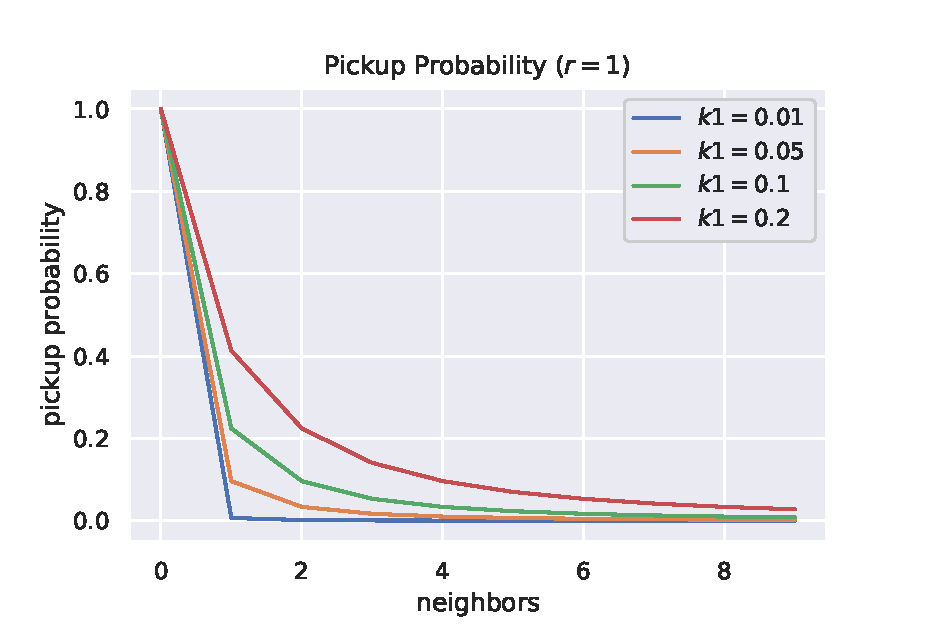
\includegraphics[width=\textwidth]{figures/aca/k1-r1.eps}
        \caption{$k_1$ vs neighbors with $r=1$}
    \end{subfigure}%
    \begin{subfigure}[t]{0.32\textwidth}
        \centering
        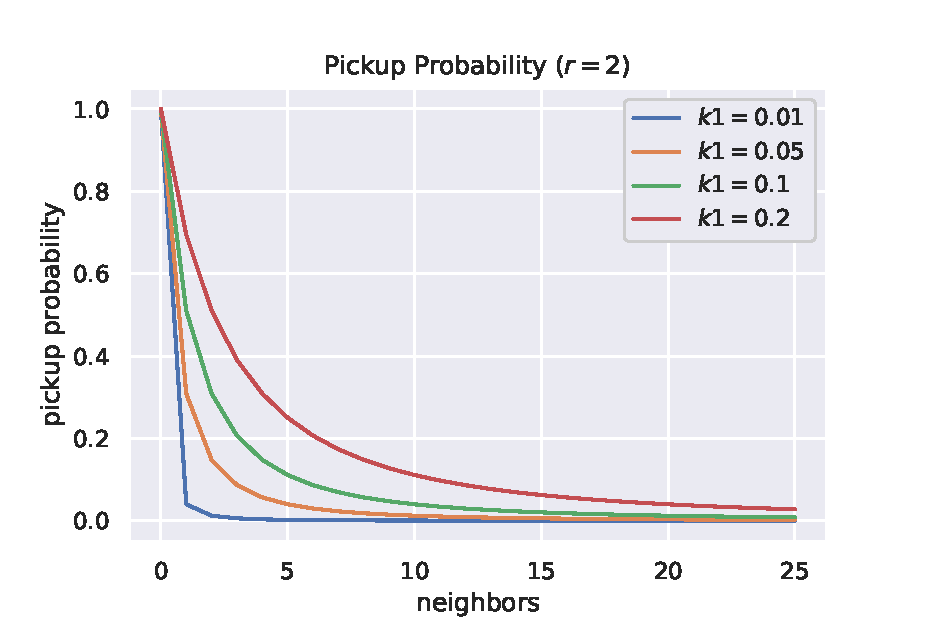
\includegraphics[width=\textwidth]{figures/aca/k1-r2.eps}
        \caption{$k_1$ vs neighbors with $r=2$}
    \end{subfigure}%
    \begin{subfigure}[t]{0.32\textwidth}
        \centering
        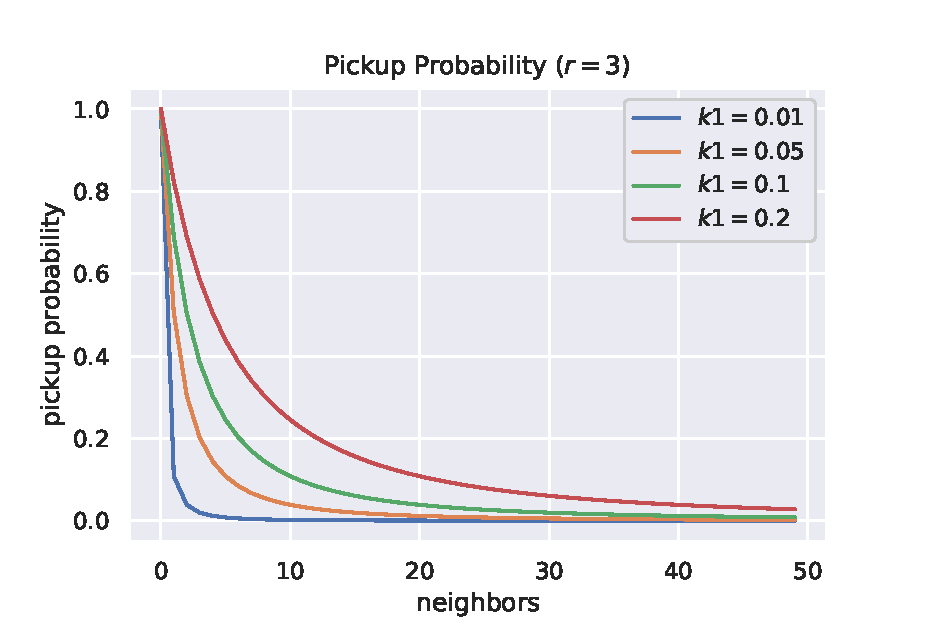
\includegraphics[width=\textwidth]{figures/aca/k1-r3.eps}
        \caption{$k_1$ vs neighbors with $r=3$}
    \end{subfigure}

    \begin{subfigure}[b]{0.32\textwidth}
        \centering
        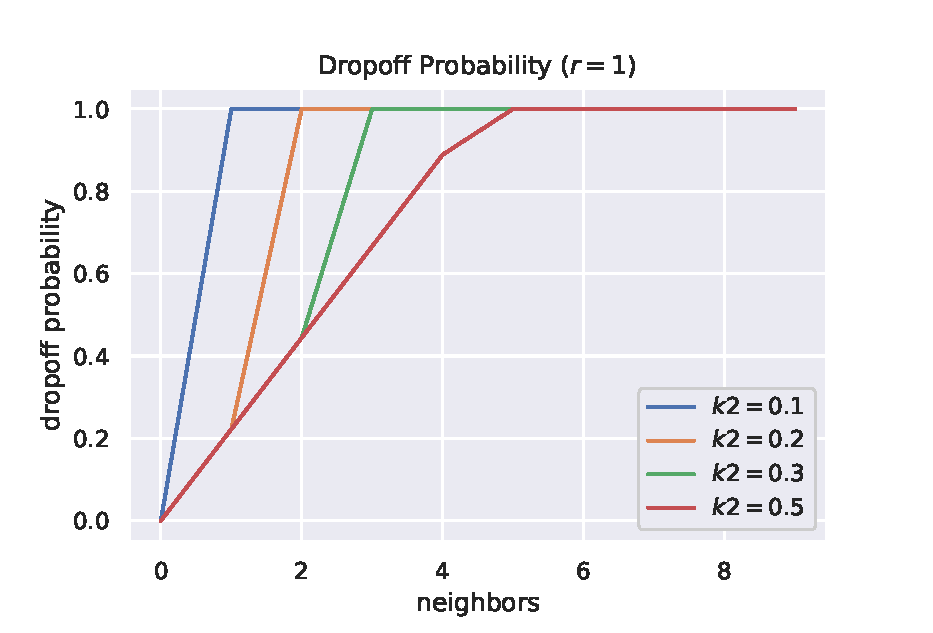
\includegraphics[width=\textwidth]{figures/aca/k2-r1.eps}
        \caption{$k_2$ vs neighbors with $r=1$}
    \end{subfigure}%
    \begin{subfigure}[b]{0.32\textwidth}
        \centering
        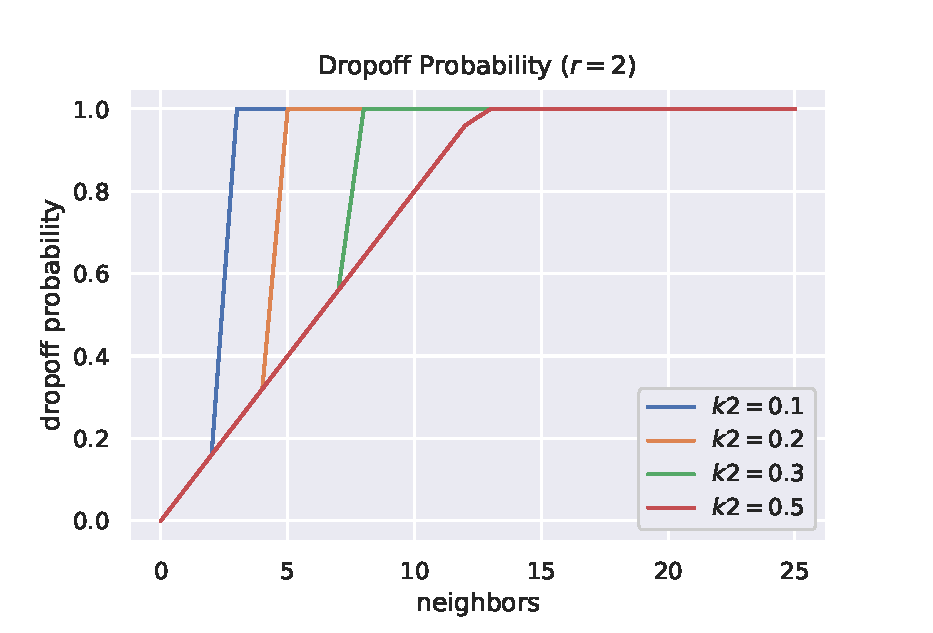
\includegraphics[width=\textwidth]{figures/aca/k2-r2.eps}
        \caption{$k_2$ vs neighbors with $r=2$}
    \end{subfigure}%
    \begin{subfigure}[b]{0.32\textwidth}
        \centering
        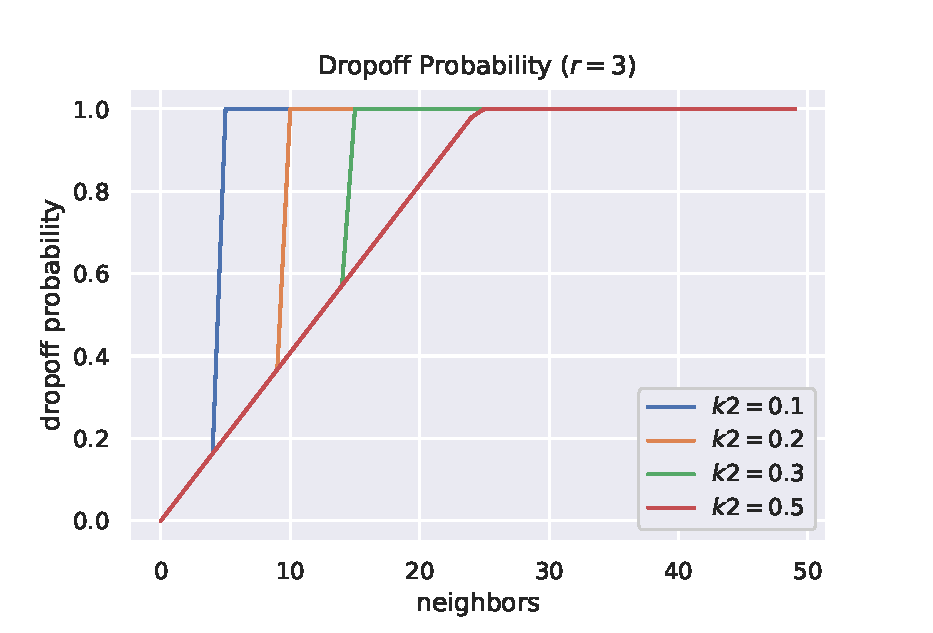
\includegraphics[width=\textwidth]{figures/aca/k2-r3.eps}
        \caption{$k_2$ vs neighbors with $r=3$}
    \end{subfigure}%
\end{figure}
\paragraph{The Number of Colors}
\paragraph{The Number of Objects}

\section{Particle Swarm Optimization}

\subsection{Statement}

Use particle swarm optimization to optimize the function
\begin{equation}
    f(x) = 2^{-2{\left(\frac{(x - 0.1)}{0.9}\right)}^2}{\big(\sin(5\pi x)\big)}^6\label{eq:pso:objective}
\end{equation}
and compare the results with those of simulated annealing from Homework 1.
\begin{figure}
    \centering
    \begin{subfigure}[b]{0.49\textwidth}
        \centering
        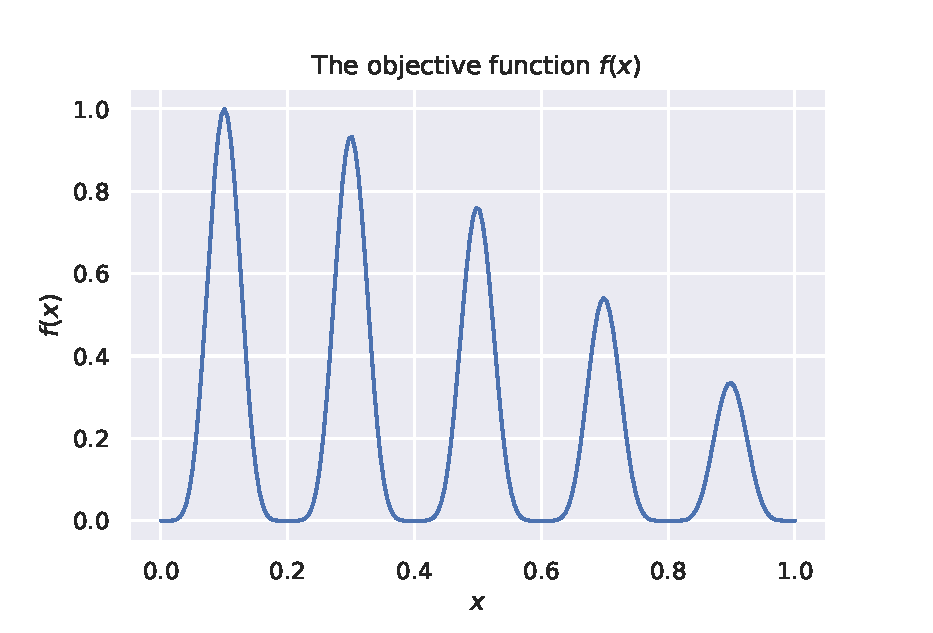
\includegraphics[width=\textwidth]{figures/pso/prob1-function.eps}
    \end{subfigure}
    \begin{subfigure}[b]{0.49\textwidth}
        \centering
        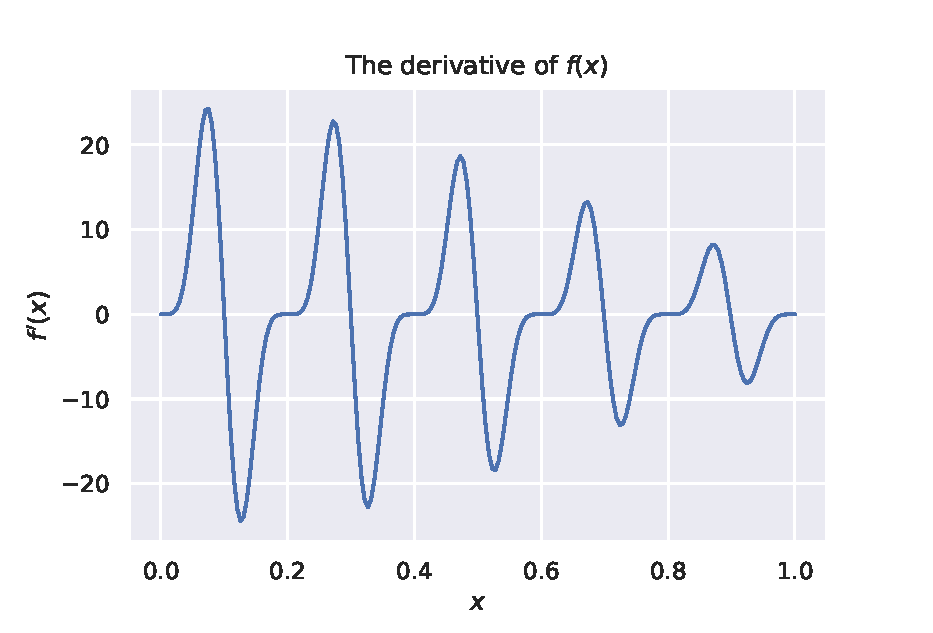
\includegraphics[width=\textwidth]{figures/pso/prob1-derivative.eps}
    \end{subfigure}
    \caption{The objective function~\ref{eq:pso:objective} and its derivative.}\label{fig:pso:objective}
\end{figure}
\autoref{eq:pso:objective} is plotted, along with its derivative, in \autoref{fig:pso:objective}.

\subsection{Method}

The standard particle swarm algorithm from the book is given in \autoref{alg:particle-swarm}.
The algorithm is tunable by the number of iterations, the acceleration constants $AC_1$ and $AC_2$, and the range of allowable velocities $[v_{\min}, v_{\max}]$.

\begin{algorithm}
    % \begin{noindent}
    \begin{algorithmic}
        \Function{PS}{$iters$, $AC_1$, $AC_2$, $v_{\min}$, $v_{\max}$}
            \State{Randomly initialize swarm $\vec{x_i} \in X$}
            \State{Randomly initialize swarm velocities $\Delta\vec{x_i}$}
            \IComment{$\Delta\vec{x_i} \in [v_{\min}, v_{\max}]$}
            \State{Let each $\vec{p_i} \gets \vec{x_i}$}
            \IComment{Best historical position for each particle}
            \State{$t \gets 1$}
            \While{$t < iters$}
                \For{$i \in \{1, \dots, particles\}$}
                    \IComment{For each particle}
                    \If{$f(\vec{x_i}) > f(\vec{p_i})$}
                        \IComment{Keep track of each particle's best position}
                        \State{$\vec{p_i} \gets \vec{x_i}$}
                    \EndIf{}
                    \State{$k \gets i$}\IComment{Arbitrary starting index}
                    \For{$j \in \{\text{neighbors of $\vec{x_i}$}\}$}
                        \IComment{Keep track of each particle's best neighbor}
                        \If{$f(\vec{p_j}) > g(\vec{p_k})$}
                            \State{$k \gets j$}
                        \EndIf{}
                    \EndFor{}
                    \State{Generate $\vec{\varphi_1}$ and $\vec{\varphi_2}$ uniformly}
                    \IComment{elementwise $\vec\varphi_i \in [0, AC]$}
                    % TODO: There's got to be a way to left justify the comment with the following
                    % line's indentation when it appears on an empty line...
                    \Statex\IComment{Linear combination of particle $i$'s historical best and neighbor's best}
                    \State{$\Delta\vec{x_i} \gets \Delta\vec{x_i} + \vec{\varphi_1} \otimes (\vec{p_i} - \vec{x_i}) + \vec{\varphi_2} \otimes (\vec{p_k} - \vec{x_i})$}
                    \State{$\Delta\vec{x_i} \in [v_{\min}, v_{\max}]$}
                    \IComment{Do not allow the velocities to explode, componentwise}
                    \State{$\vec{x_i} \gets \vec{x_i} + \Delta\vec{x_i}$}
                \EndFor{}
                \State{$t \gets t + 1$}
            \EndWhile{}
            \State\Return{$X$}
        \EndFunction{}
    \end{algorithmic}
    % \end{noindent}
    \caption{The standard Particle Swarm (PS) optimization algorithm}\label{alg:particle-swarm}
\end{algorithm}

The book states that the acceleration constants should equal 4.1. That is,
\[AC_1 + AC_2 = 4.1\]
with $AC_1 = AC_2 = 2.05$.
The acceleration constants are used to draw the vectors of weights $\vec{\varphi_1}$ and $\vec{\varphi_2}$ from a uniform distribution of $[0, AC_1]$ and $[0, AC_2]$ respectively.
Note that the $\otimes$ symbol is elementwise multiplication.

The update step
\begin{equation}
    \Delta\vec{x_i} \gets \Delta\vec{x_i} + \vec{\varphi_1} \otimes (\vec{p_i} - \vec{x_i}) + \vec{\varphi_2} \otimes (\vec{p_k} - \vec{x_i})\label{eq:pso:update}
\end{equation}
considers the direction towards the particle's best known position, and the best known position of its neighbors.
It updates its velocity as a randomly weighted linear combination of those directions.

There are several variants of \autoref{alg:particle-swarm} to consider.
One such variation is to consider, not the each best historical position of each particle's neighbors, but the best historical position of the entire swarm.
This difference is shown in \autoref{alg:particle-swarm-variant}.

\begin{algorithm}
    % \begin{noindent}
    \begin{algorithmic}
        \Function{PS-variant}{$iters$, $AC_1$, $AC_2$, $v_{\min}$, $v_{\max}$}
            \State{Randomly initialize swarm $\vec{x_i} \in X$}
            \State{Randomly initialize swarm velocities $\Delta\vec{x_i}$}
            \IComment{$\Delta\vec{x_i} \in [v_{\min}, v_{\max}]$}
            \State{Let each $\vec{p_i} \gets \vec{x_i}$}
            \IComment{Best historical position for each particle}
            \State{Let $\vec{p} \gets$ best $\vec{x_i} \in X$}
            \IComment{Swarm's best historical position}
            \State{$t \gets 1$}
            \While{$t < iters$}
                \For{$i \in \{1, \dots, particles\}$}
                    \IComment{For each particle}
                    \If{$f(\vec{x_i}) > f(\vec{p_i})$}
                        \IComment{Keep track of each particle's best position}
                        \State{$\vec{p_i} \gets \vec{x_i}$}
                    \EndIf{}
                    \If{$f(\vec{x_i}) > f(\vec{p})$}
                        \IComment{Update the swarm's best position}
                        \State{$\vec{p} \gets \vec{x_i}$}
                    \EndIf{}
                    \State{Generate $\vec{\varphi_1}$ and $\vec{\varphi_2}$ uniformly}
                    \IComment{elementwise $\vec\varphi_i \in [0, AC]$}
                    % TODO: There's got to be a way to left justify the comment with the following
                    % line's indentation when it appears on an empty line...
                    \Statex\IComment{Linear combination of particle $i$'s historical best and
                        swarm's best}
                    \State{$\Delta\vec{x_i} \gets \Delta\vec{x_i} + \vec{\varphi_1} \otimes (\vec{p_i} - \vec{x_i}) + \vec{\varphi_2} \otimes (\vec{p} - \vec{x_i})$}
                    \State{$\Delta\vec{x_i} \in [v_{\min}, v_{\max}]$}
                    \IComment{Do not allow the velocities to explode, componentwise}
                    \State{$\vec{x_i} \gets \vec{x_i} + \Delta\vec{x_i}$}
                \EndFor{}
                \State{$t \gets t + 1$}
            \EndWhile{}
            \State\Return{$X$}
        \EndFunction{}
    \end{algorithmic}
    % \end{noindent}
    \caption{A variant Particle Swarm optimization algorithm}\label{alg:particle-swarm-variant}
\end{algorithm}

We implemented \autoref{alg:particle-swarm-variant} to solve the given problem.

\subsection{Implementation}

The implementation of a single iteration of \autoref{alg:particle-swarm-variant} is straightforward.

\begin{minted}{python}
    def update(self, func):
        """Perform one iteration of optimization."""
        for i, particle in enumerate(self.particles):
            if func(x) > func(self.history[i]):
                self.history[i] = particle
            if func(x) > func(self.best):
                self.best = particle

            phi1 = np.random.uniform(low=0, high=self.AC1, size=1)
            phi2 = np.random.uniform(low=0, high=self.AC2, size=1)

            self.velocities[i] += phi1 * (self.history[i] - particle) + phi2 * (self.best - particle)
            # Clip the velocities.
            self.velocities[i] = min(self.vmax, max(self.vmin, self.velocities[i]))
            self.particles[i] += self.velocities[i]
            # Clip the positions.
            self.particles[i] = min(self.xmax, max(self.xmin, self.particles[i]))
\end{minted}

It \textit{should} be straightforward to parallelize this to update each particle at once, or in batches.
However, to do so correctly, the swarm's best known position, \mintinline{python}{self.best} should be guarded with a mutex.
Further, multithreading in Python often yields little-to-no improvement in runtime, because every single object in Python is guarded by the Global Interpreter Lock (GIL).
Threading is still useful in networking or file operation contexts, threading is eschewed for performing CPU-bound work in favor of multiprocessing.
The difficulty in using multiple processes for this task is that they have no shared memory, which increases the amount of communication overhead to a point we are unlikely to see a big performance benefit for this particular problem.

Not to mention that extremely small numbers of particles were still effective in optimizing \autoref{eq:pso:objective} due to the size of the feasible region.

Note that this implementation is strictly one-dimensional.
Additional work must be done to optimize functions of multiple variables.
To work in more than one dimension,
\begin{itemize}
    \item $\varphi_1$ and $\varphi_2$ should have the same dimension as each particle.
    \item Each particle velocity should be a tuple of velocities --- one for each dimension.
    \item The particle velocity and position clipping should be done componentwise.
\end{itemize}

Running the PSO algorithm for multiple iterations is equally straightforward.

\begin{minted}{python}
    def optimize(self, func, iters, animate=False):
        """Optimize the given function for `iters` iterations."""
        b = np.argmax(func(self.particles))
        self.best = self.particles[b]

        for i in range(iters):
            self.update(func)

            if animate and i % 5 == 0:
                self.plot(func, blocking=False)

        return self.best
\end{minted}

As in the first problem, we implemented our solution in such as way as to allow us to play with a large number of tweakable parameters.
All of the parameters are adjustable via commandline arguments shown below.

\begin{minted}{text}
    $ ./prob2.py --help
    usage: prob2.py [-h] [--xmin XMIN] [--xmax XMAX] [--ac1 AC1] [--ac2 AC2]
                    [--vmin VMIN] [--vmax VMAX] [--particles PARTICLES]
                    [--iterations ITERATIONS] [--animate] [--headless]

    Optimize a function with a particle swarm.

    optional arguments:
    -h, --help              show this help message and exit
    --xmin XMIN             The lower domain boundary.
    --xmax XMAX             The upper domain boundary.
    --ac1 AC1               Acceleration constant for the particle history component.
    --ac2 AC2               Acceleration constant for the swarm history component.
    --vmin VMIN             The particle velocity lower bound.
    --vmax VMAX             The particle velocity upper bound.
    --particles PARTICLES, -p PARTICLES
                            The number of particles in the swarm.
    --iterations ITERATIONS, -i ITERATIONS
                            The number of iterations to use.
    --animate               Animate the swarm's progress.
    --headless              A headless mode for profiling.
\end{minted}

Note that considerable more work would need to be done, as above, to make this wrapper script handle multivariate objective functions.
The difficulty lies in specifying the feasible region to optimize over, using commandline arguments.

Setting the objective function to optimize is less easy to do from the commandline,\footnote{In a secure fashion. It's possible to use \mintinline{python}{eval()} or \mintinline{python}{ast.literal_eval()}, but both of these methods make this author queasy.}
so the \mintinline{python}{func(x)} function in the `prob2.py' script must be edited.

\subsection{Results}
\subsubsection{Hill Climbing}
Recall\footnote{Or let us make the recollection for you.} from Homework 1 that hill climbing struggles with ``spiky'' functions.
\autoref{fig:pso:hill-climbing-results} shows the results from several independent runs of the hill climbing algorithm on the objective function \autoref{eq:pso:objective}.

\begin{figure}[H]
    \centering
    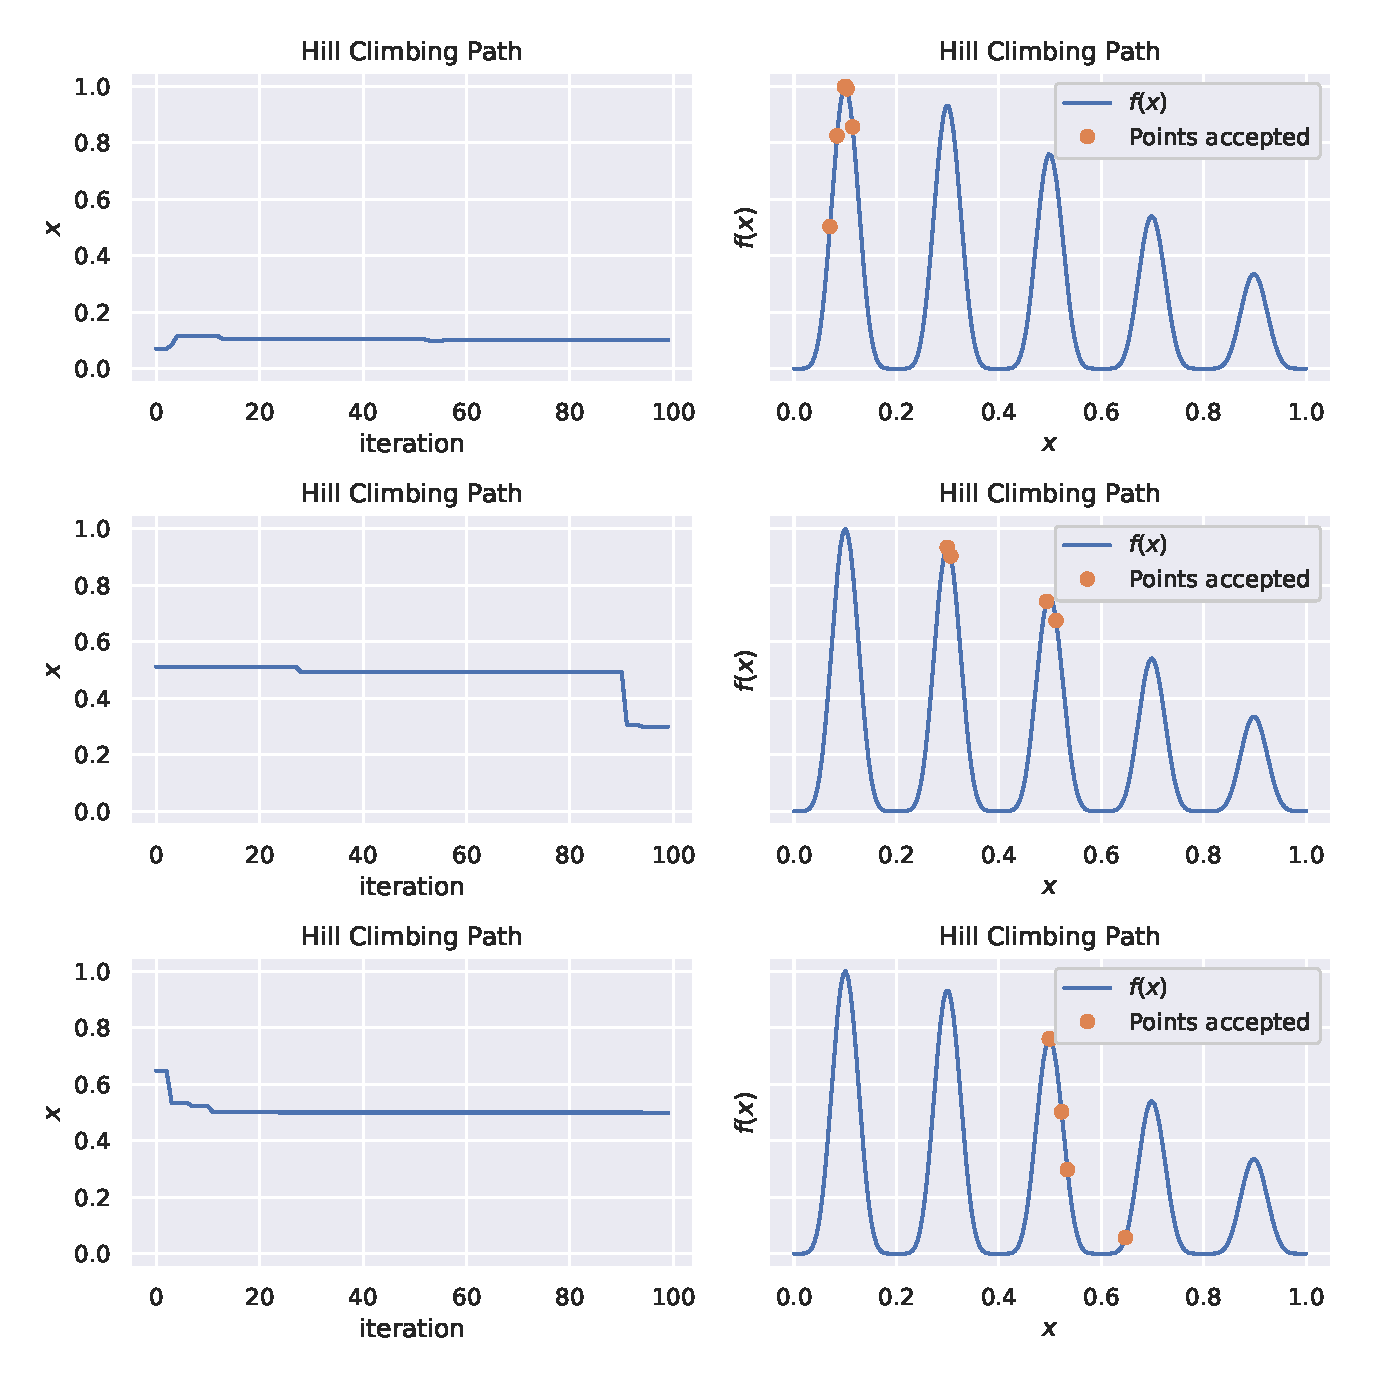
\includegraphics[width=\textwidth]{figures/pso/prob1-hill-climbing-results.eps}
    \caption{Results from three successive runs of the hill climbing algorithm.}\label{fig:pso:hill-climbing-results}
\end{figure}

Running the randomly-initialized hill climbing algorithm multiple times in parallel and taking the best result works okay, as long as the number of parallel runs is proportional to the density of the spikes in the feasible region.
\autoref{fig:pso:hill-climbing-parallel} shows the aggregated results of several parallel runs of the iterated hill climbing algorithm.

From this we can immediately see that there is quite a bit in the variance of multiple runs.
The success of the hill climbing algorithm depends entirely on the its random initialization.

\begin{figure}[H]
    \centering
    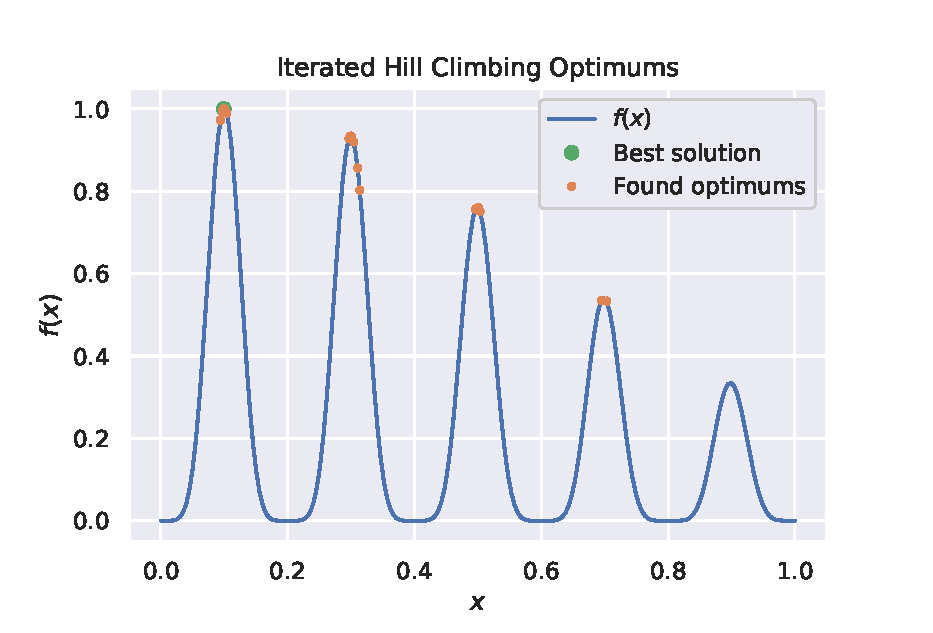
\includegraphics{figures/pso/prob1-hill-climbing-solution.eps}
    \caption{Results from multiple runs of the hill climbing algorithm in parallel.}\label{fig:pso:hill-climbing-parallel}
\end{figure}

\subsubsection{Simulated Annealing}
Recall also that simulated annealing worked \textit{much} better.
\autoref{fig:pso:simulated-annealing-results} shows a steady peak-to-peak trend from the simulated annealing algorithm, because it accepts enough random solutions to explore non-local space, but over time cools down enough to settle to a reasonable solution.

\begin{figure}[H]
    \centering
    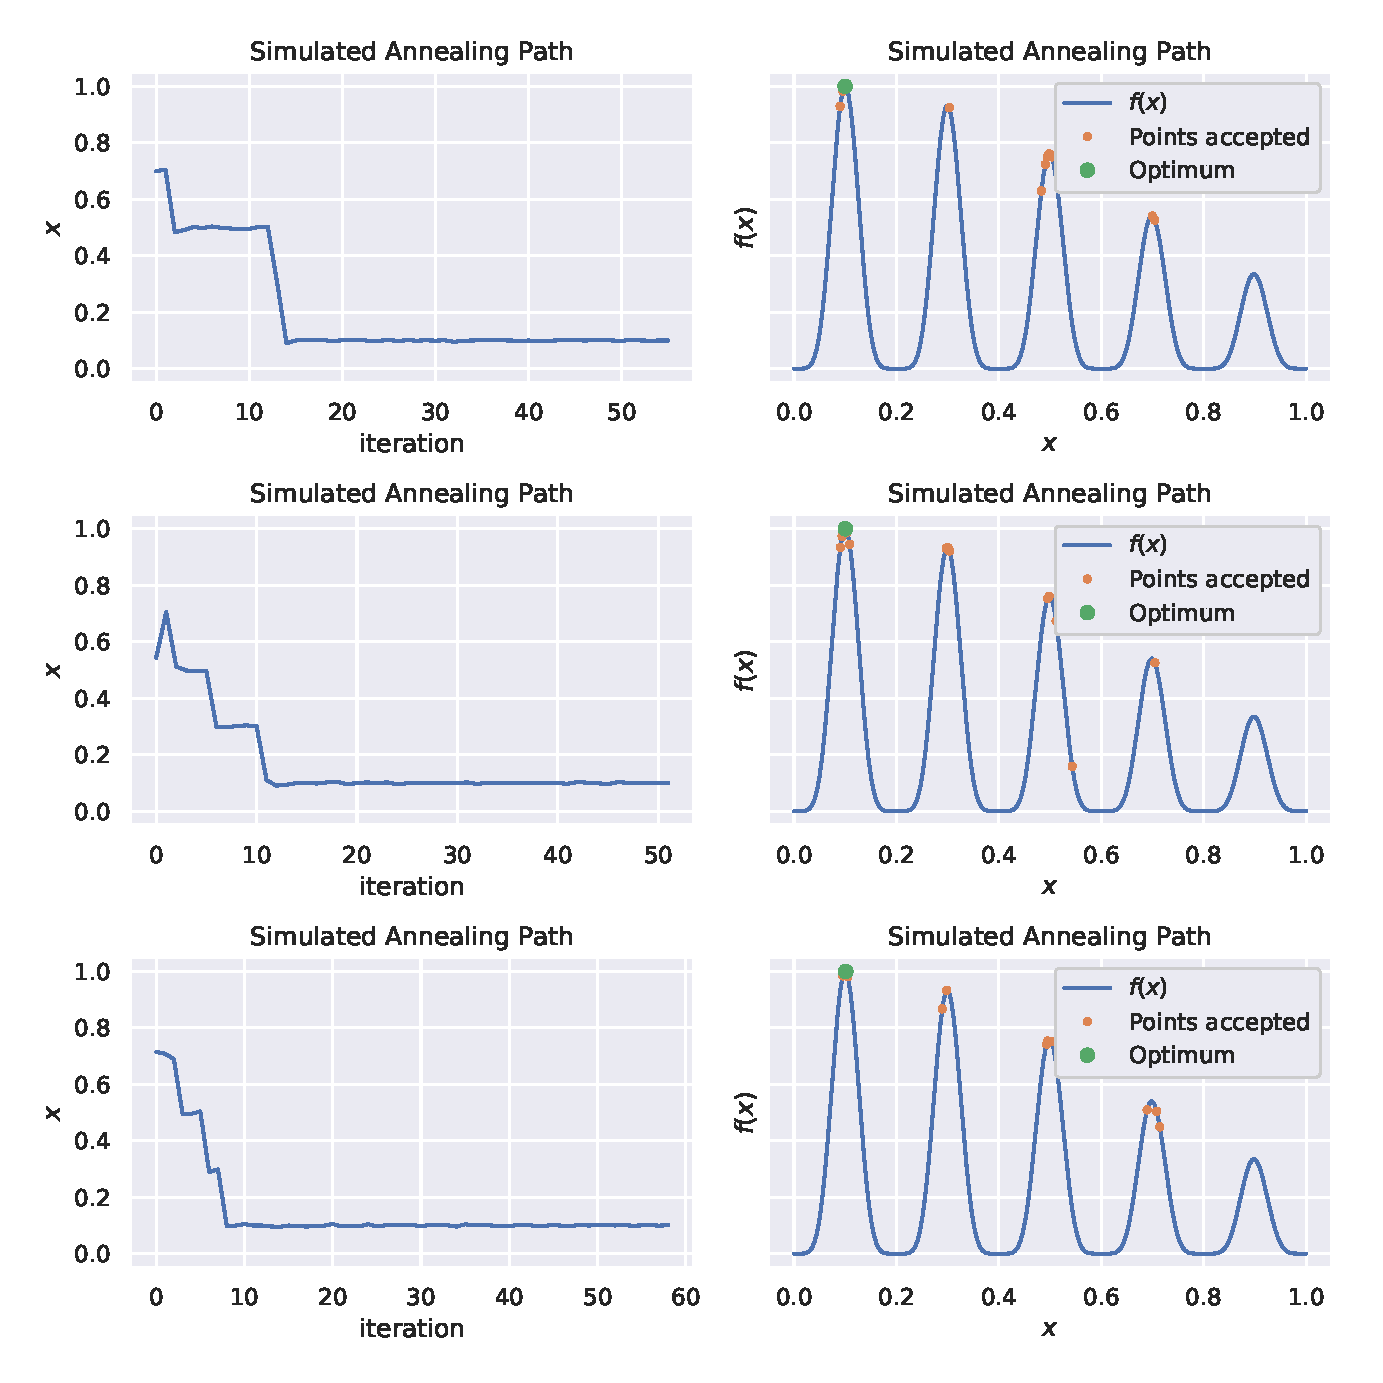
\includegraphics[width=\textwidth]{figures/pso/prob1-simulated-annealing-results.eps}
    \caption{Results from three successive runs of the simulated annealing algorithm.}\label{fig:pso:simulated-annealing-results}
\end{figure}

\autoref{fig:pso:simulated-annealing-parallel} is much more illuminating; not only does the simulated annealing algorithm not find non-global solutions, each iterated run settled down to exactly the same solution.

\begin{figure}[H]
    \centering
    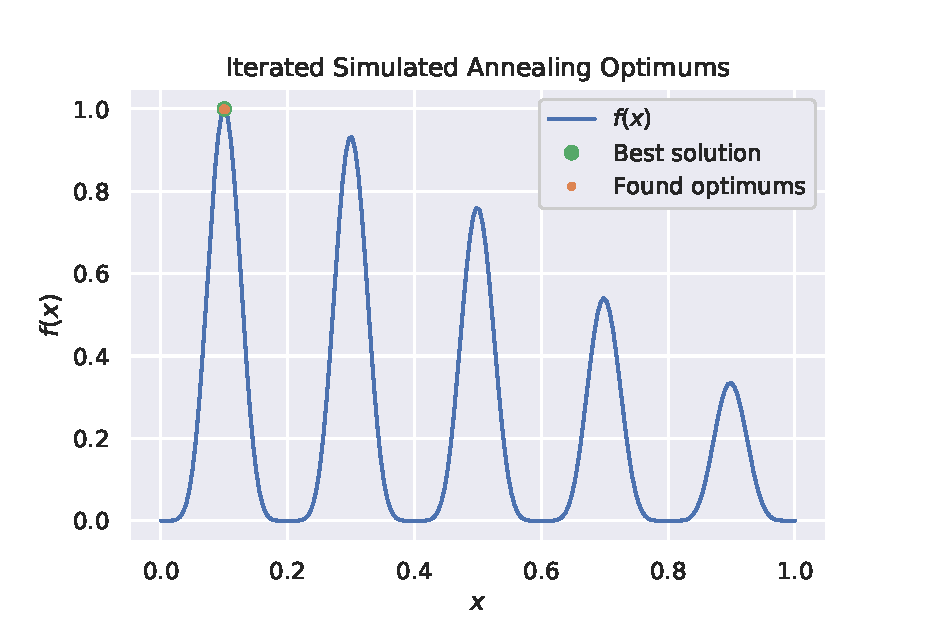
\includegraphics{figures/pso/prob1-simulated-annealing-solutions.eps}
    \caption{Results from multiple runs of the simulated annealing algorithm in parallel.}\label{fig:pso:simulated-annealing-parallel}
\end{figure}

\subsubsection{Particle Swarm}
As mentioned above, we enabled the modification of multiple different tweakable parameters via commandline arguments.
Below we discuss the impacts of several such parameters.

We arbitrarily chose default parameters, and as mentioned below, we can get much better performance by applying some amount of intelligence.

\paragraph{The Swarm Size} The easiest and most obvious parameter to tweak for the particle swarm algorithm is the number of particles to use.
With our poorly chosen default parameters, simply increasing the number of particles was sufficient to guarantee convergence to the solution.

This is an acceptable method due to the size and complexity of the problem.
We are optimizing a well-behaved univariate function over a small feasible region with a relatively small number of spikes.
All the swarm needs to do to converge to the solution is begin with at least one particle on the largest spike.

\begin{figure}[H]
    \centering
    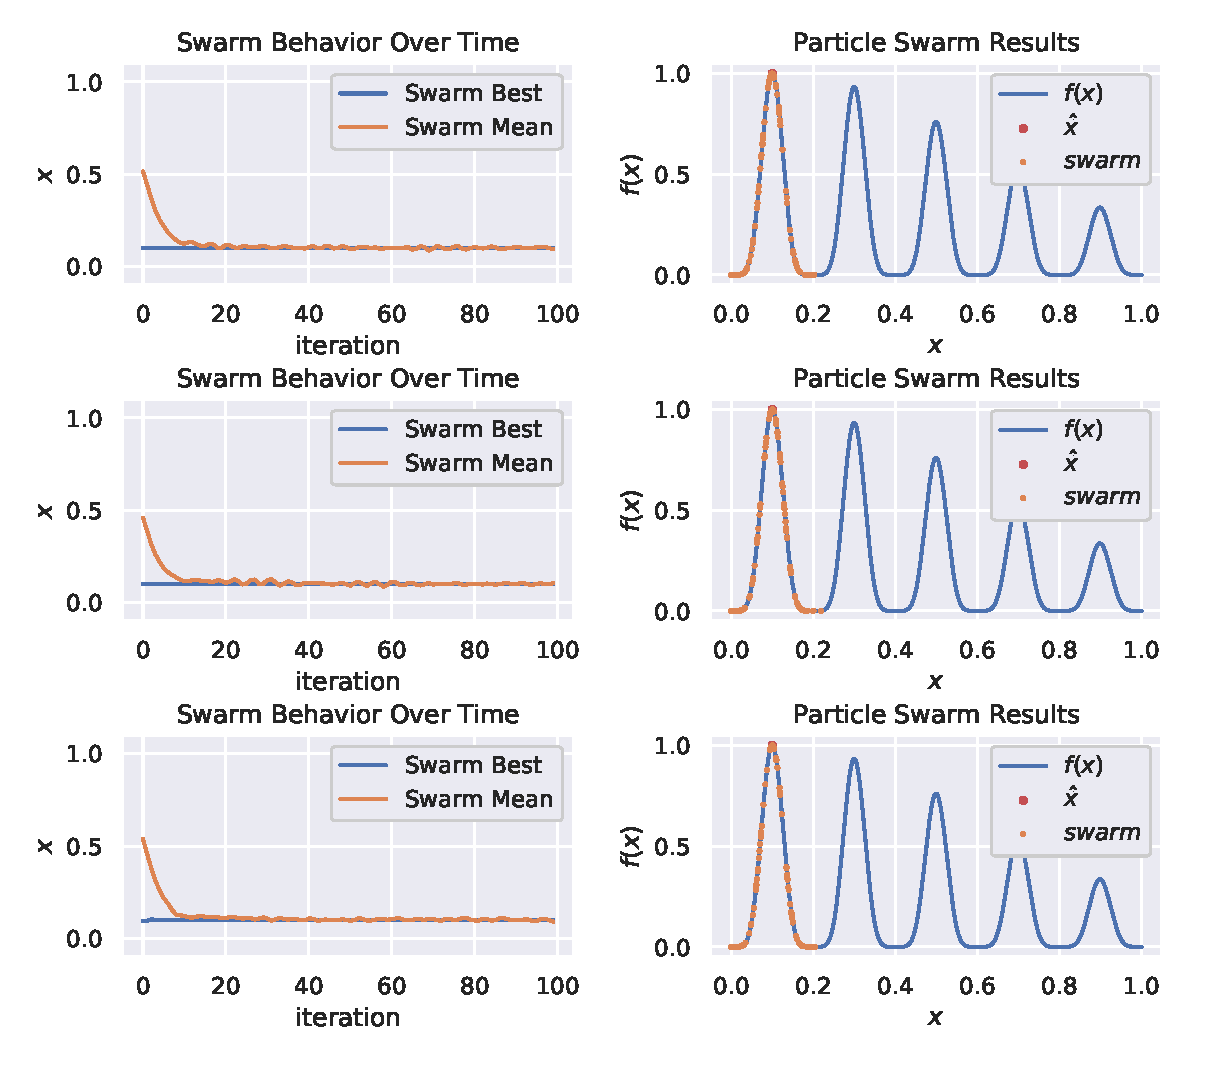
\includegraphics[width=\textwidth]{figures/pso/pso-100-particles.eps}
    \caption{The PSO algorithm with default parameters and 100 particles}\label{fig:pso:100-particles}
\end{figure}

Figures~\ref{fig:pso:100-particles} and~\ref{fig:pso:5-particles} shows the results with 100 and 5 particles respectively.

\begin{figure}[H]
    \centering
    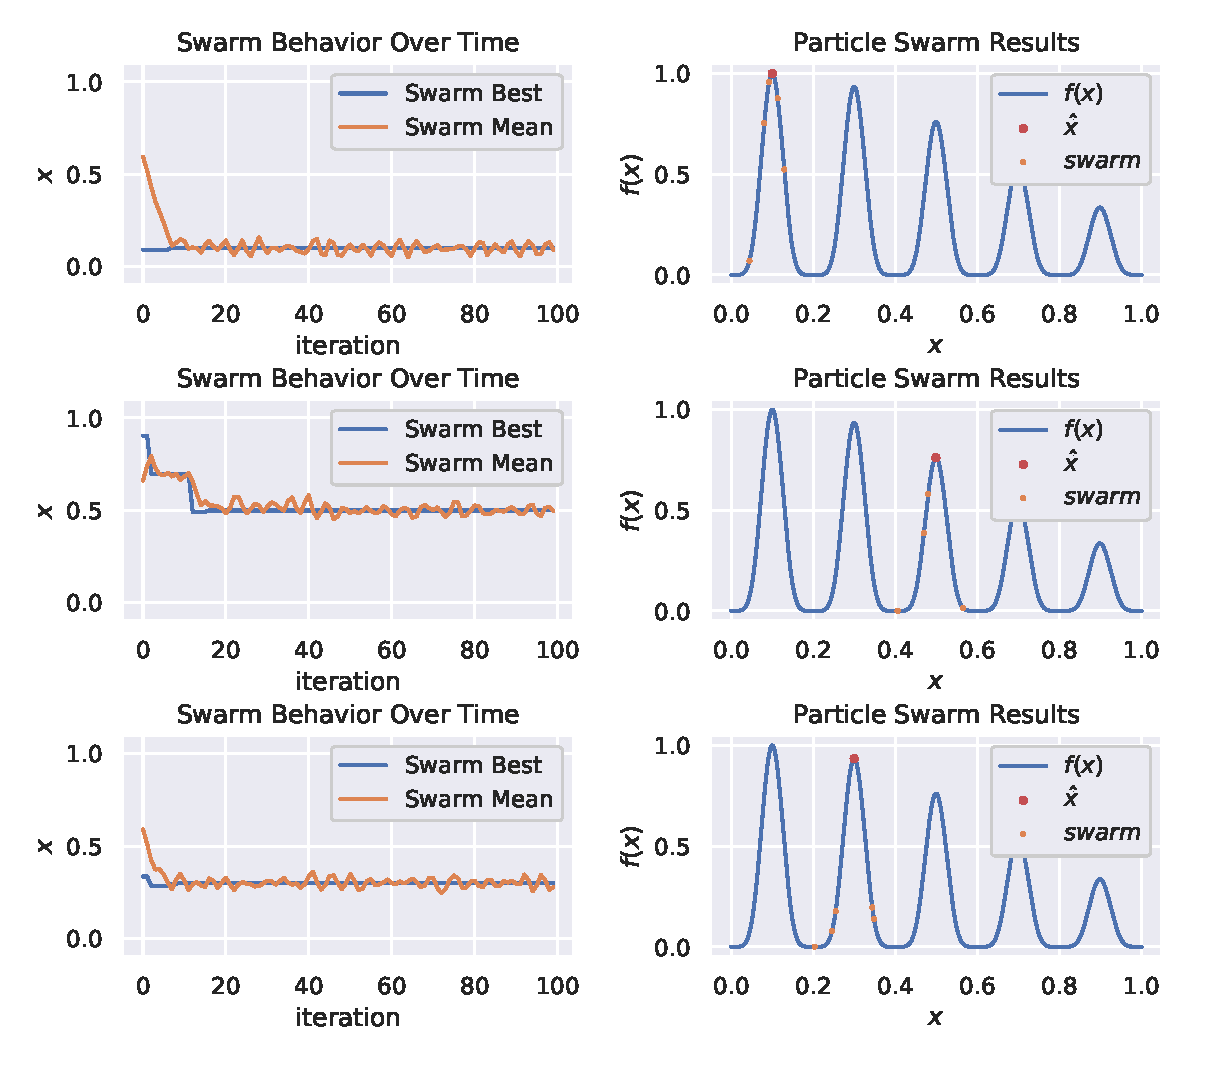
\includegraphics[width=\textwidth]{figures/pso/pso-5-particles.eps}
    \caption{The PSO algorithm with default parameters and 5 particles}\label{fig:pso:5-particles}
\end{figure}

Observe from \autoref{fig:pso:100-particles} that the swarm appears densest at the peak and troughs of the first spike.
When we animated the progress of the swarm, most of the particles seemed to accumulated \textit{between} spikes, which was surprising.

Notice also that the swarm is uniformly initialized throughout the domain, so the swarm mean is exactly that --- the mean of the $[0, 1]$ domain.

\paragraph{The Velocity Bounds $[v_{\min}, v_{\max}]$} The next parameter we chose to experiment with was the velocity bounds.
The velocity bounds restrict the maximum step a particle may take after its direction has been determined.
What we saw during animation of the swarm with small numbers of particles was that the swarm would clump around a single spike and never explore any of the other spikes.
Increasing the maximum allowable step size to allow stepping from one spike to another fixed the local behavior we saw.

This might be because particles were now free to overshoot their planned trajectories, and overshooting enabled the exploration of other regions of the search space.

\begin{figure}[H]
    \centering
    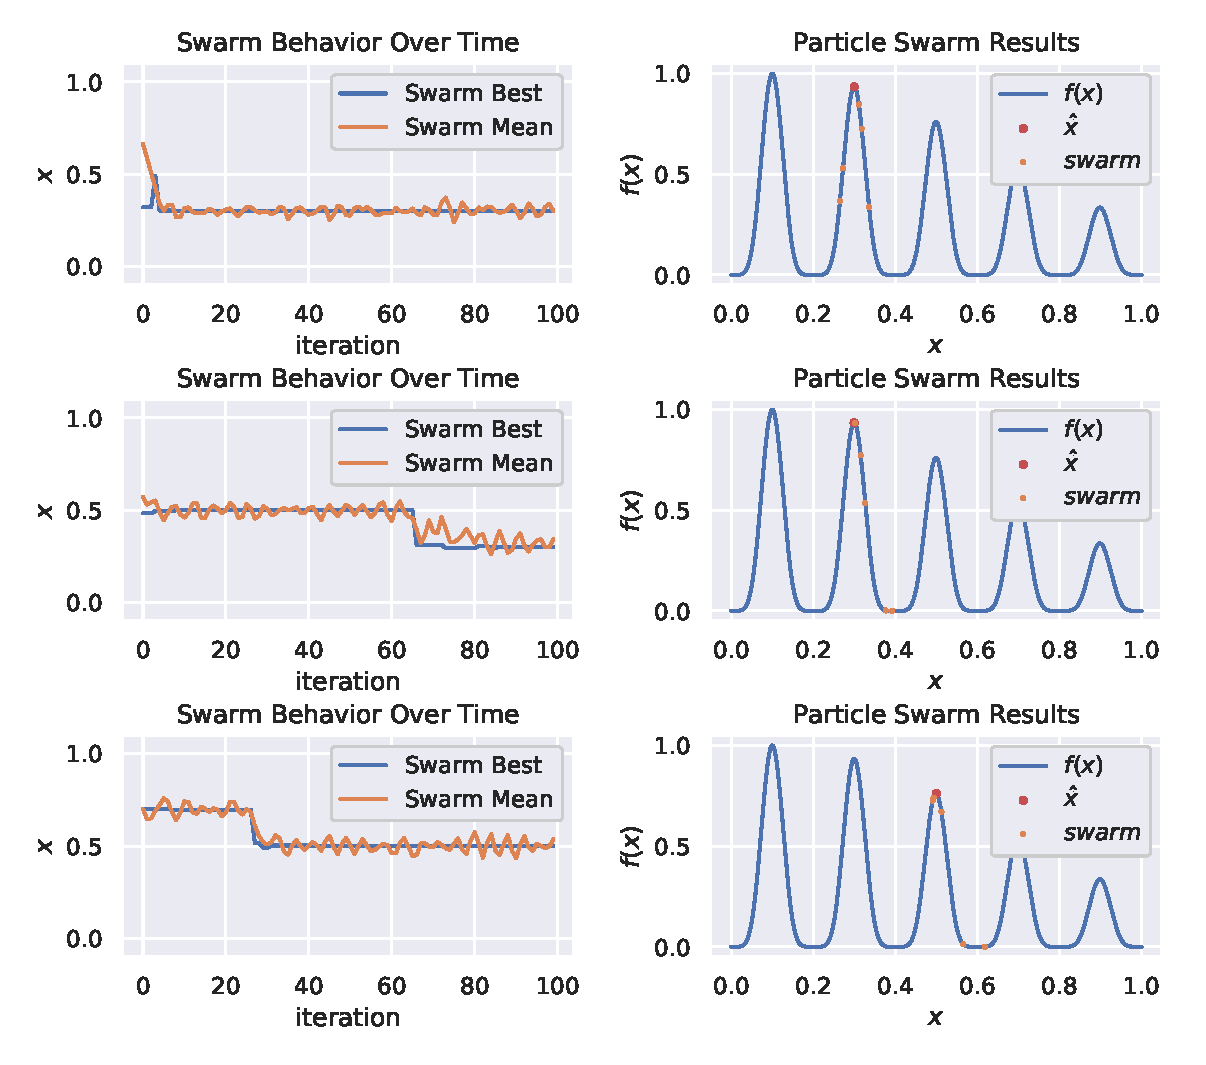
\includegraphics[width=\textwidth]{figures/pso/pso-v01.eps}
    \caption{Results with the default velocity bounds $[-0.1, 0.1]$}\label{fig:pso-vmin-01-vmax-01}
\end{figure}

\autoref{fig:pso-vmin-01-vmax-01} shows the PSO results with the default bounds we chose of $[-0.1, 0.1]$.
From this, we can see that the swarm mean does not jump from spike to spike nearly enough to find the global optimum.

\begin{figure}[H]
    \centering
    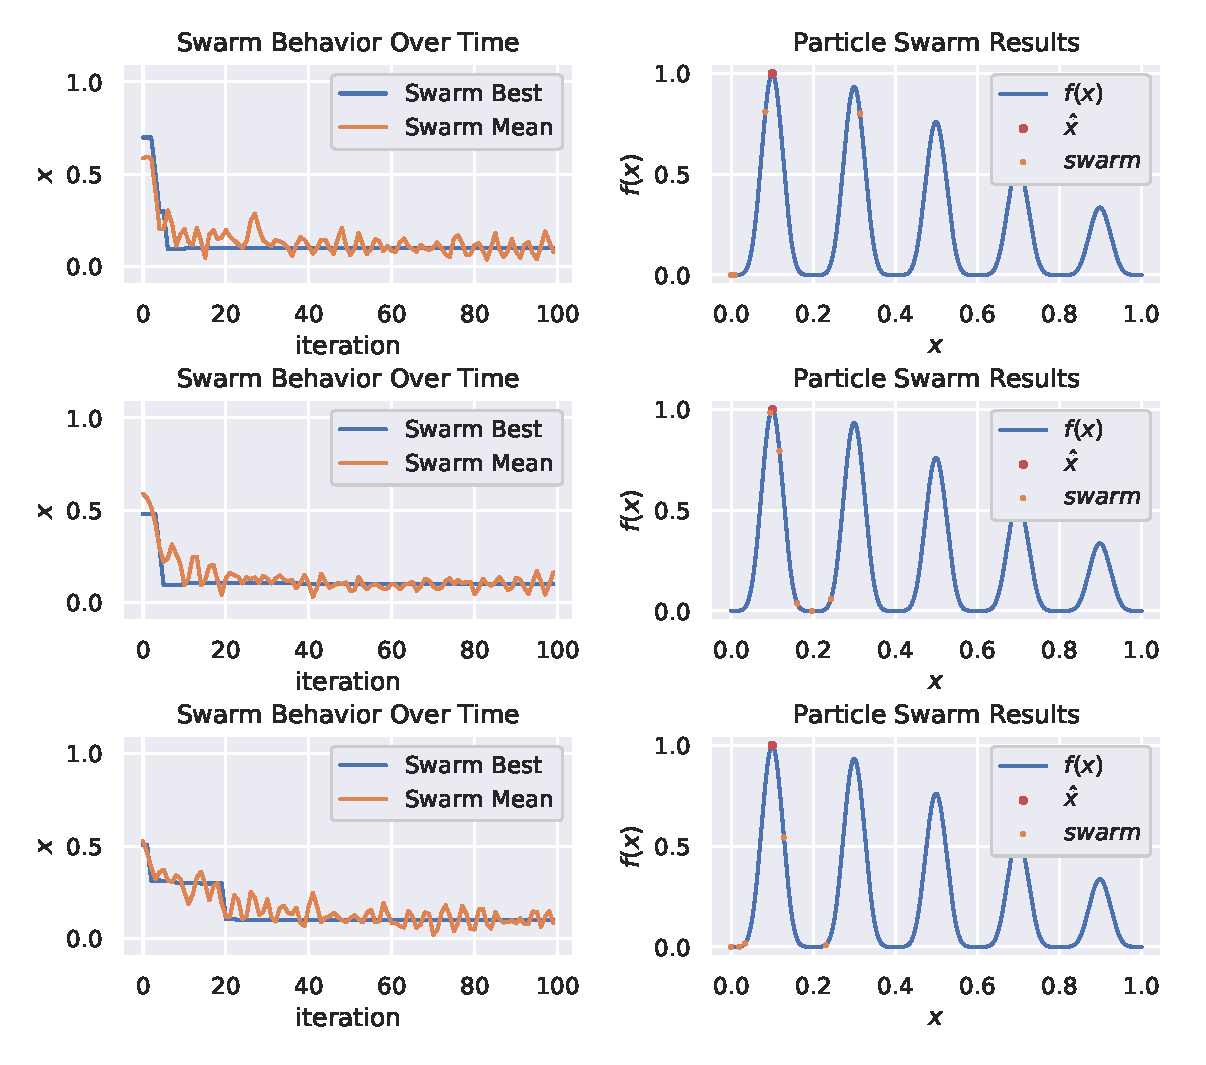
\includegraphics[width=\textwidth]{figures/pso/pso-v021.eps}
    \caption{Results with the velocity bounds $[-0.2, 0.2]$}\label{fig:pso-vmin-02-vmax-02}
\end{figure}

Enabling larger jumps in particle positions on each iteration readily fixed this problem.
\autoref{fig:pso-vmin-02-vmax-02} shows the results with bounds $[-0.2, 0.2]$.

We can see that the swarm jumps to the biggest spike quite early, and spends most of its time centered around the spike's peak.
This is the desired behavior.
Notice again, however, that the actual positions of the particles seemed to prefer the valleys \textit{between} the peaks, rather than the peaks themselves.

\begin{figure}[H]
    \centering
    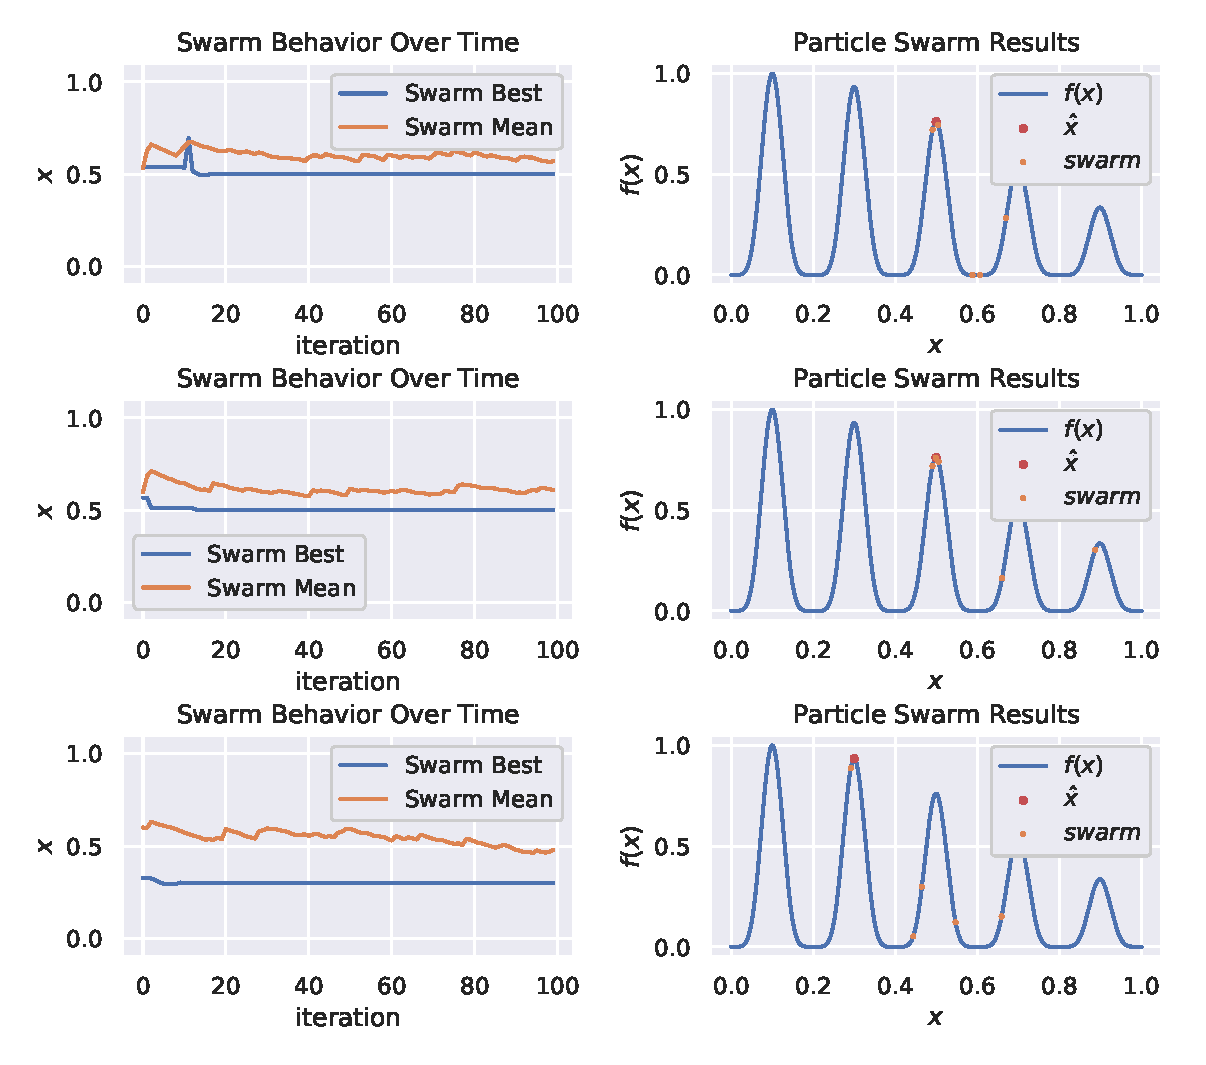
\includegraphics[width=\textwidth]{figures/pso/pso-v001-v02.eps}
    \caption{Results with the velocity bounds $[-0.01, 0.2]$}\label{fig:pso-vmin-001-vmax-02}
\end{figure}

We can bias the swarm to one direction or the other.
That is, we can use global information about the shape of the plot to push the swarm left or right.
\autoref{fig:pso-vmin-001-vmax-02} shows the results of using velocity bounds $[-0.01, 0.2]$, which
biases the swarm to the right --- which is the opposite of what we'd like.
We have, in effect, prevented the swarm from moving left at all.

It's difficult to see, but \autoref{fig:pso-vmin-001-vmax-02} also shows that the swarm is located to the right of the warm's best historical position.
This is expected from the plot of the swarm's mean and it's best location.

\begin{figure}[H]
    \centering
    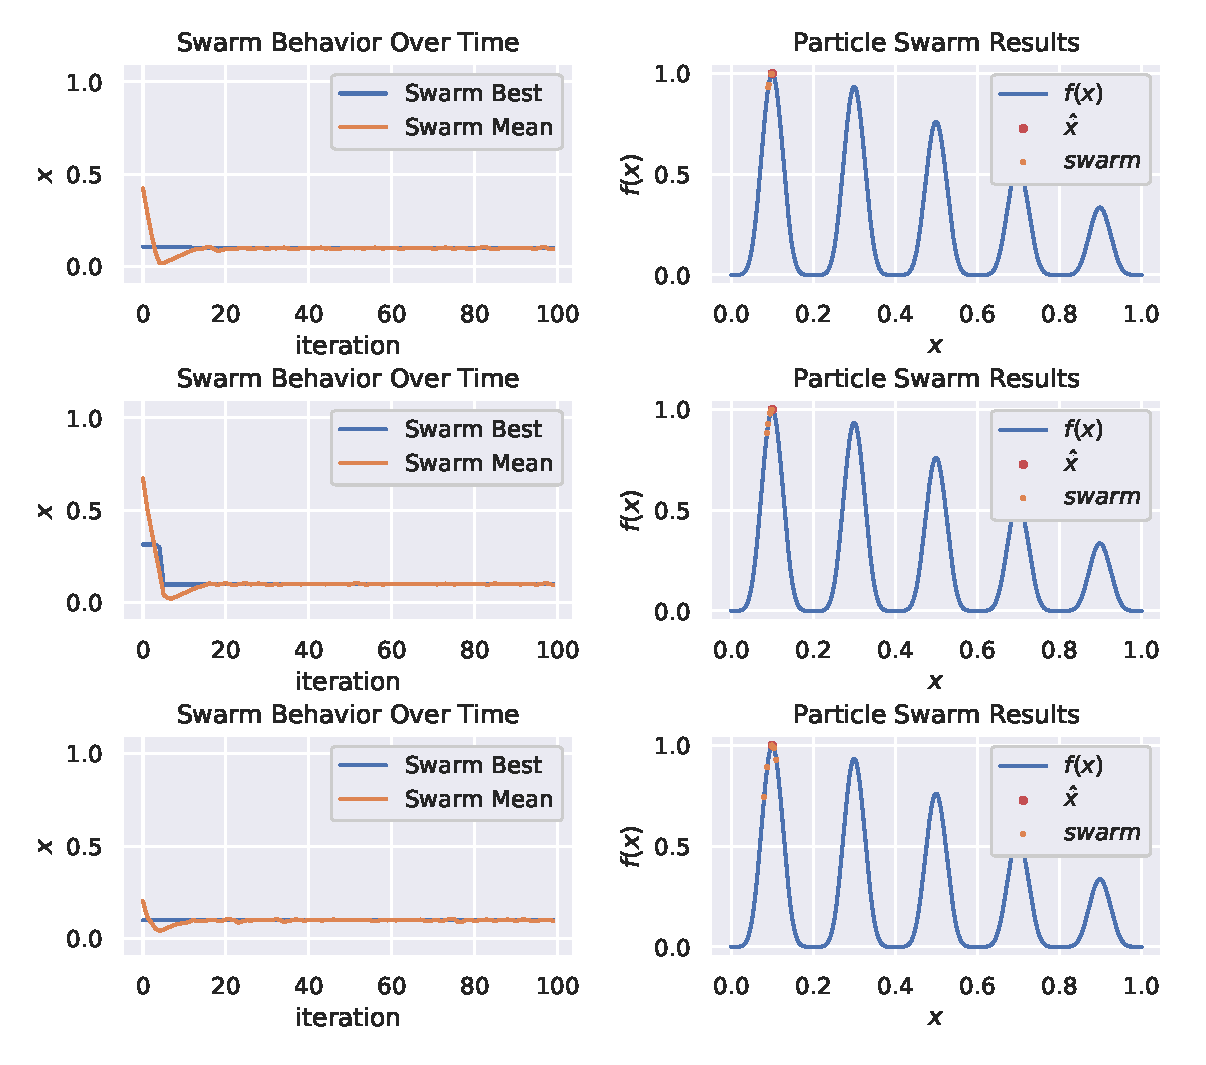
\includegraphics[width=\textwidth]{figures/pso/pso-v20-v001.eps}
    \caption{Results with the velocity bounds $[-0.2, 0.01]$}\label{fig:pso-vmin-02-vmax-001}
\end{figure}

\autoref{fig:pso-vmin-02-vmax-001} shows the results of the swarm biased in the opposite direction, with velocity bounds $[-0.2, 0.01]$.
We see an immediate pull to the left on the swarm centroid, and relatively little oscillation\footnote{This in itself is remarkable, and I'm sure would make perfect sense if one were to analyze the swarm's behavior as a system of differential equations. However, this author is suspicious of dynamical systems in general, and the mere thought of pursuing this unfortunate stray idea any farther is enough to cause heart palpitations.} after it corrects itself.

It is interesting that biasing the swarm to the right consistently forced the swarm's mean to be well above the solution, but biasing the swarm to the right forced the swarm's mean \textit{to} the solution, with little-to-no oscillation.

This time, as opposed to previous results, the particles have avoided the valleys in preference of the peaks.
This is remarkable, and has a perfectly reasonable explanation, but this is left as a simple exercise to the sophisticated reader.

\paragraph{The Acceleration Constants $AC_1$ and $AC_2$} Playing with both acceleration and velocity was revealing.

\begin{figure}[H]
    \centering
    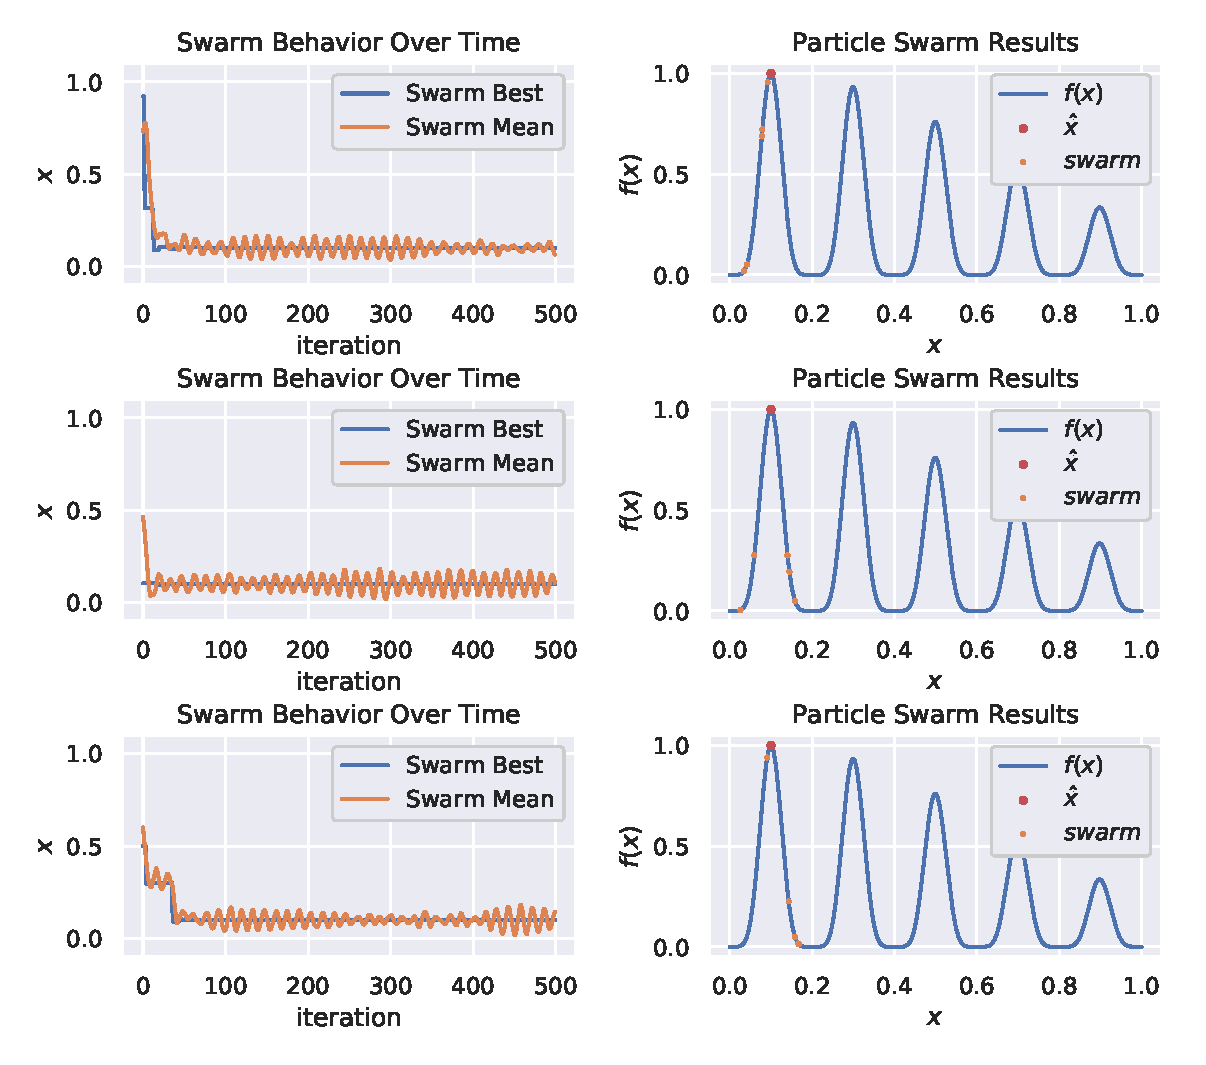
\includegraphics[width=\textwidth]{figures/pso/pso-sinusoids.eps}
    \caption{Them there's some sinusoids}\label{fig:pso:sinusoids}
\end{figure}

Different configurations of velocity and acceleration resulted in different oscillatory behavior.
This is completely unsurprising from a dynamical systems standpoints, where some configurations might be underdamped, overdamped, etc.

However, as mentioned, this author is suspicious of dynamical systems and refuses to make a claim other than ``Them there's some sinusoids''.
We were able to get results, and even some good results from the particle swarm optimization algorithm.
There's no need to perform anything so mathochistic as a dynamical systems analysis of the swarm behavior.

Note that much of the oscillatory behavior observed in this experimentation can be damped by using a swarm with more particles.

\begin{figure}[H]
    \centering
    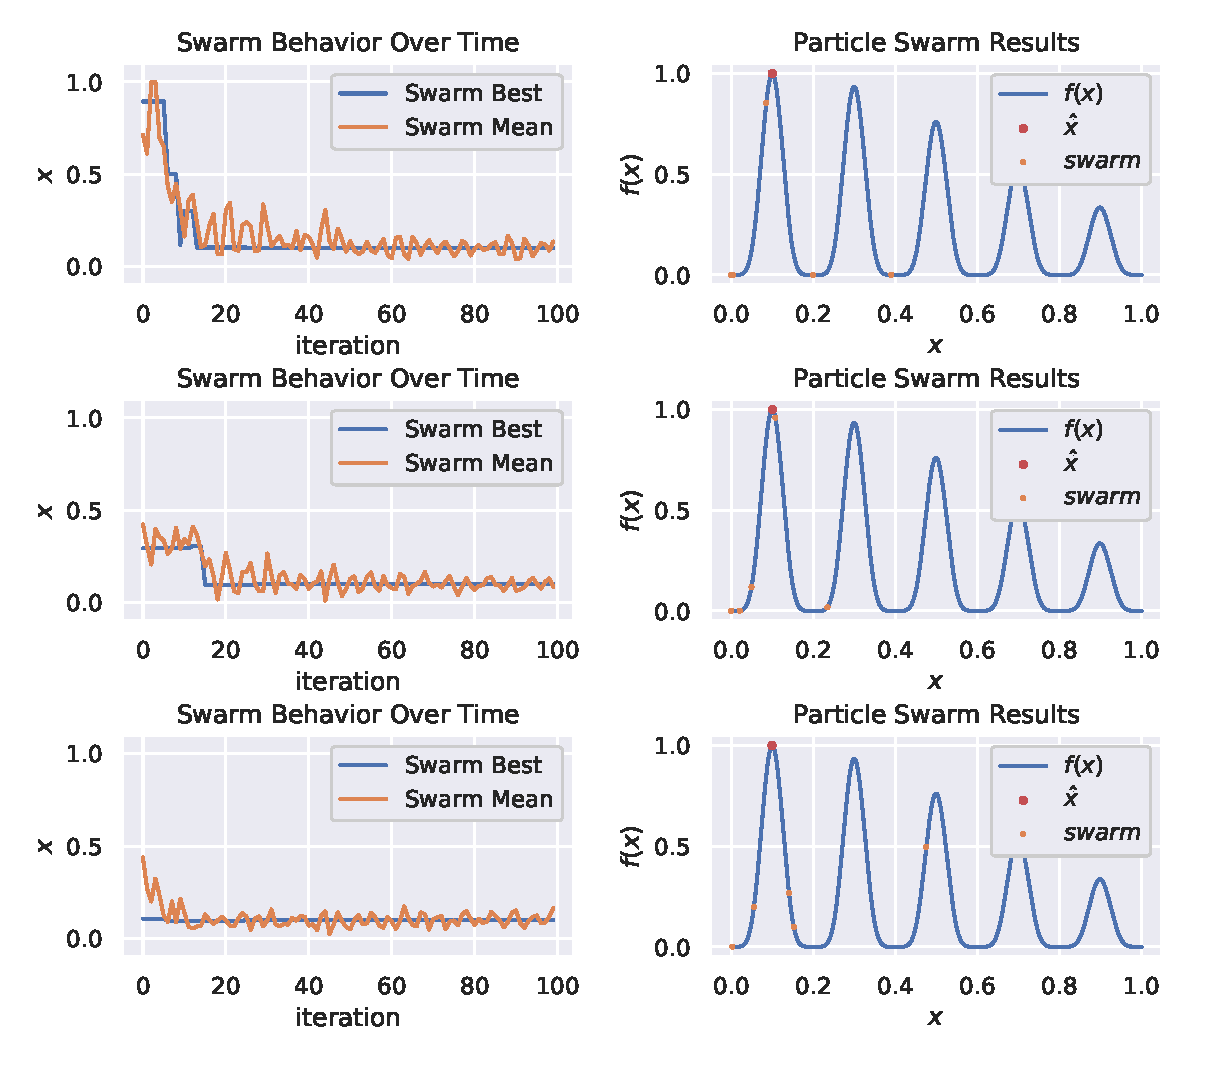
\includegraphics[width=\textwidth]{figures/pso/pso-high-vel-high-accel.eps}
    \caption{High velocity, high acceleration.}\label{fig:pso:high-vel-high-accel}
\end{figure}

Using high velocities and high accelerations means that the particles are jumping around much farther distances with every iteration.
The result is a less cohesive and more sparse swarm.
Yet a beneficial consequence is that the swarm explores more of the search space, resulting in more consistent results.

\begin{figure}[H]
    \centering
    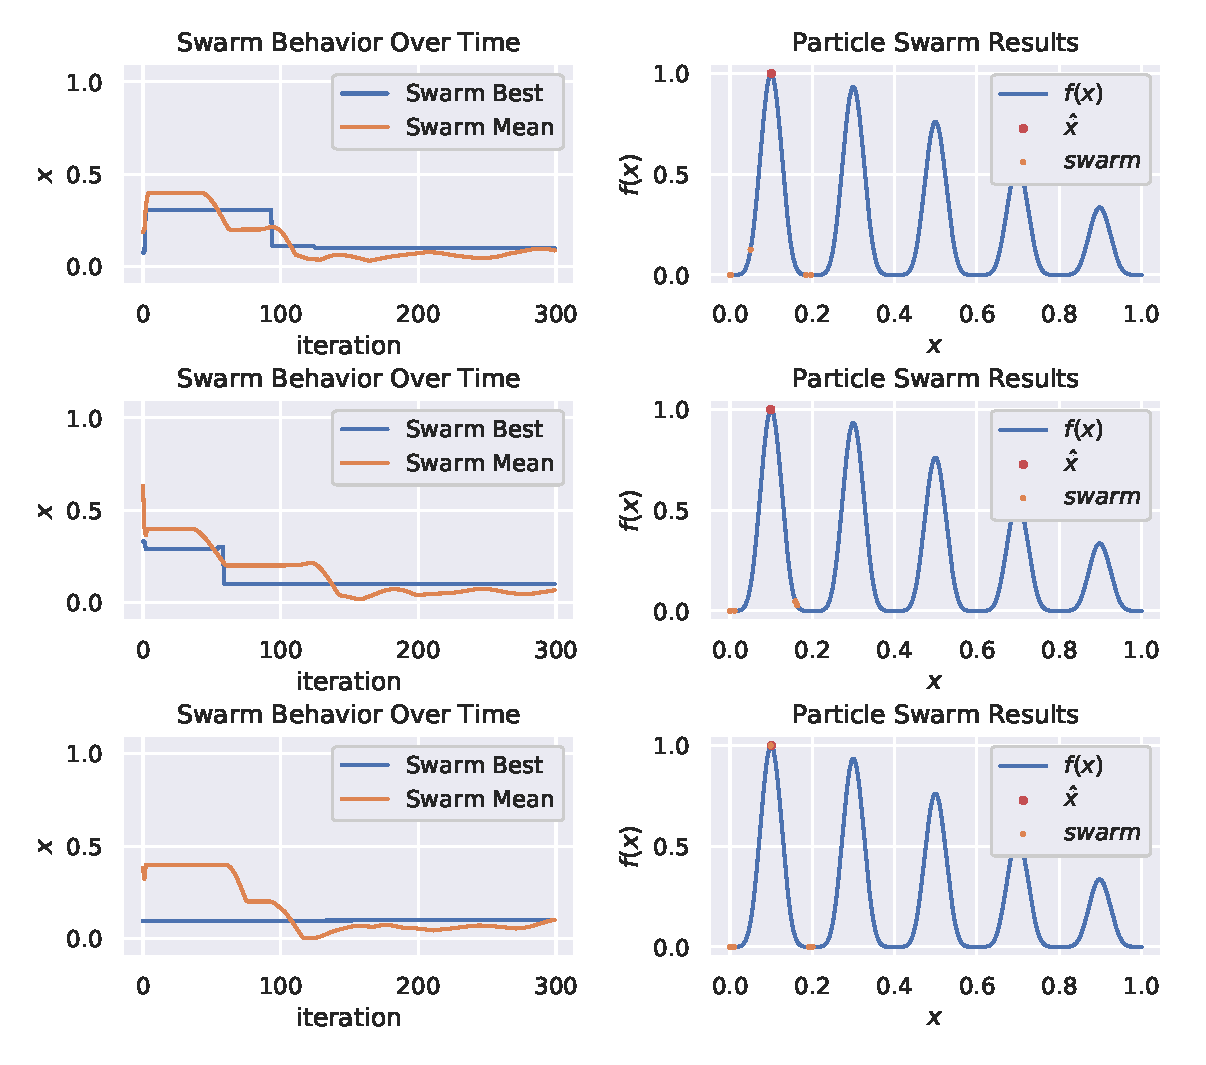
\includegraphics[width=\textwidth]{figures/pso/pso-high-vel-low-accel.eps}
    \caption{High velocity, low acceleration.}\label{fig:pso:high-vel-low-accel}
\end{figure}

Using high velocities with low acceleration results in a swarm that consistently overshoots are requires correction.
It is also necessary to run the algorithm for more iterations to settle down to a more reasonable solution.
We recommend avoiding this configuration.

\begin{figure}[H]
    \centering
    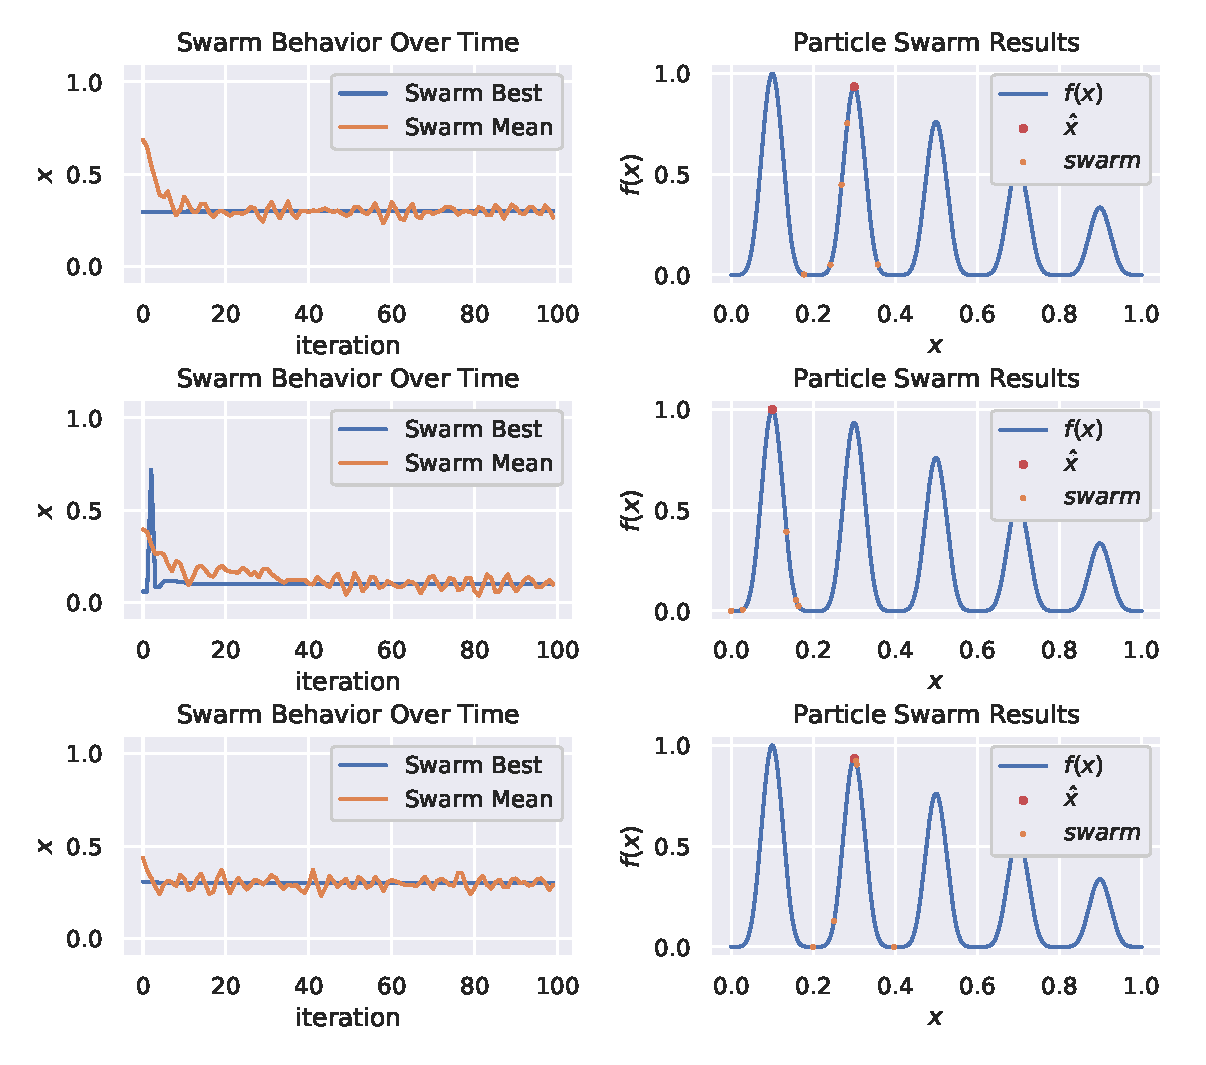
\includegraphics[width=\textwidth]{figures/pso/pso-low-vel-high-accel.eps}
    \caption{Low velocity, high acceleration.}\label{fig:pso:low-vel-high-accel}
\end{figure}

Using low velocity with a high acceleration also has undesirable results.
This is the default configuration we used in previous analysis --- a default velocity bound of $[-0.1, 0.1]$ with acceleration constants $AC_1 = AC_2 = 2$.
We recommend avoiding this configuration as well.

\begin{figure}[H]
    \centering
    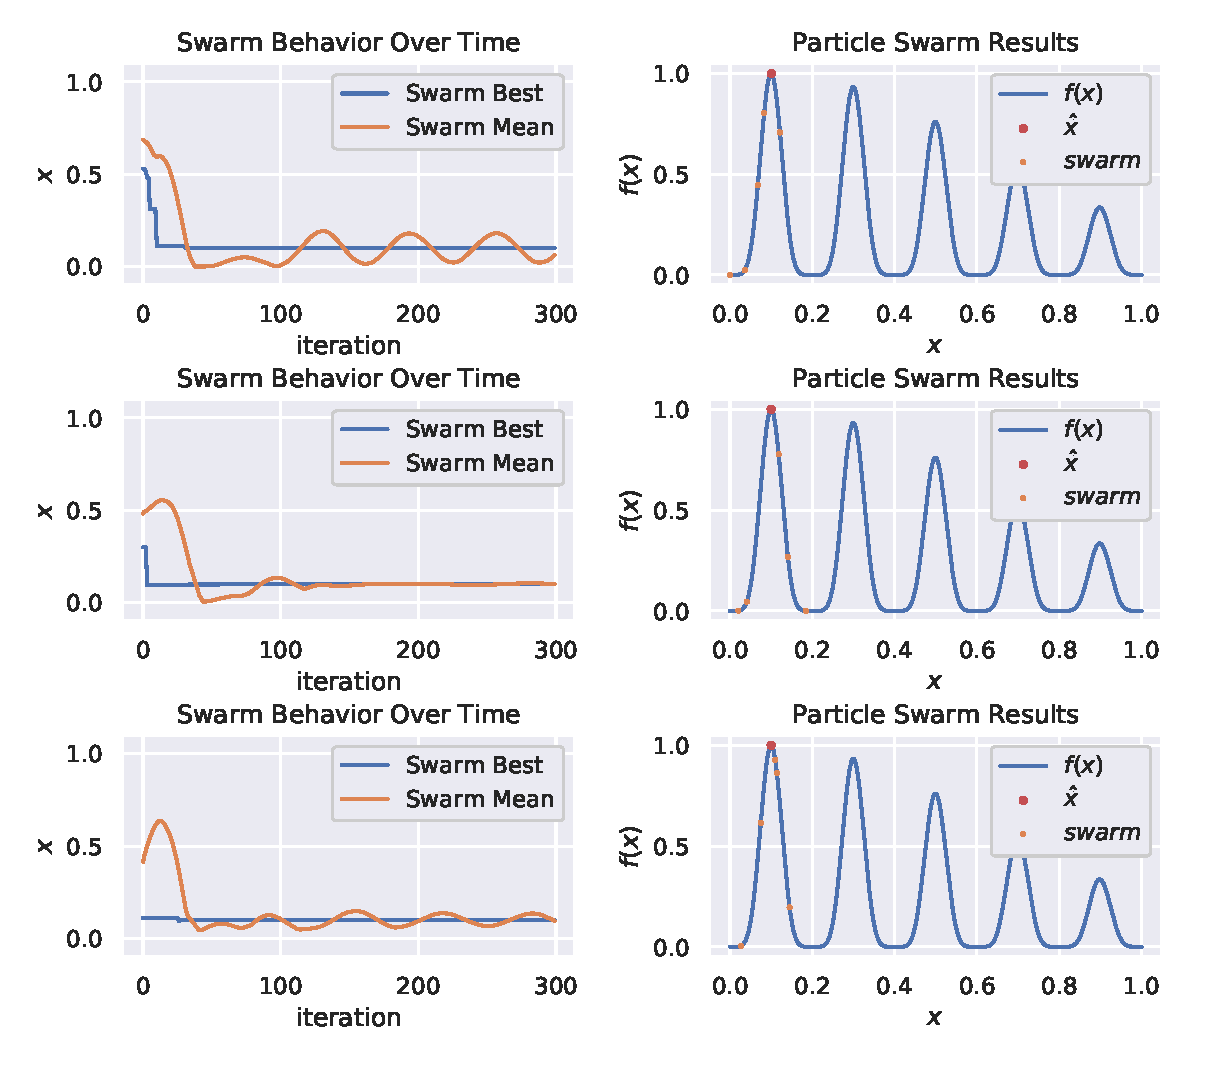
\includegraphics[width=\textwidth]{figures/pso/pso-low-vel-low-accel.eps}
    \caption{Low velocity, low acceleration.}\label{fig:pso:low-vel-low-accel}
\end{figure}

Using low velocity with low acceleration is more oscillatory than with high velocities and low acceleration.
This is because using low accelerations results in a more cohesive swarm that moves together in a tighter packed bunch.
This can be beneficial --- the swarm can move faster throughout the fitness landscape --- yet it also produces more oscillation because the swarm overshoots and has to correct itself.

\begin{figure}[H]
    \centering
    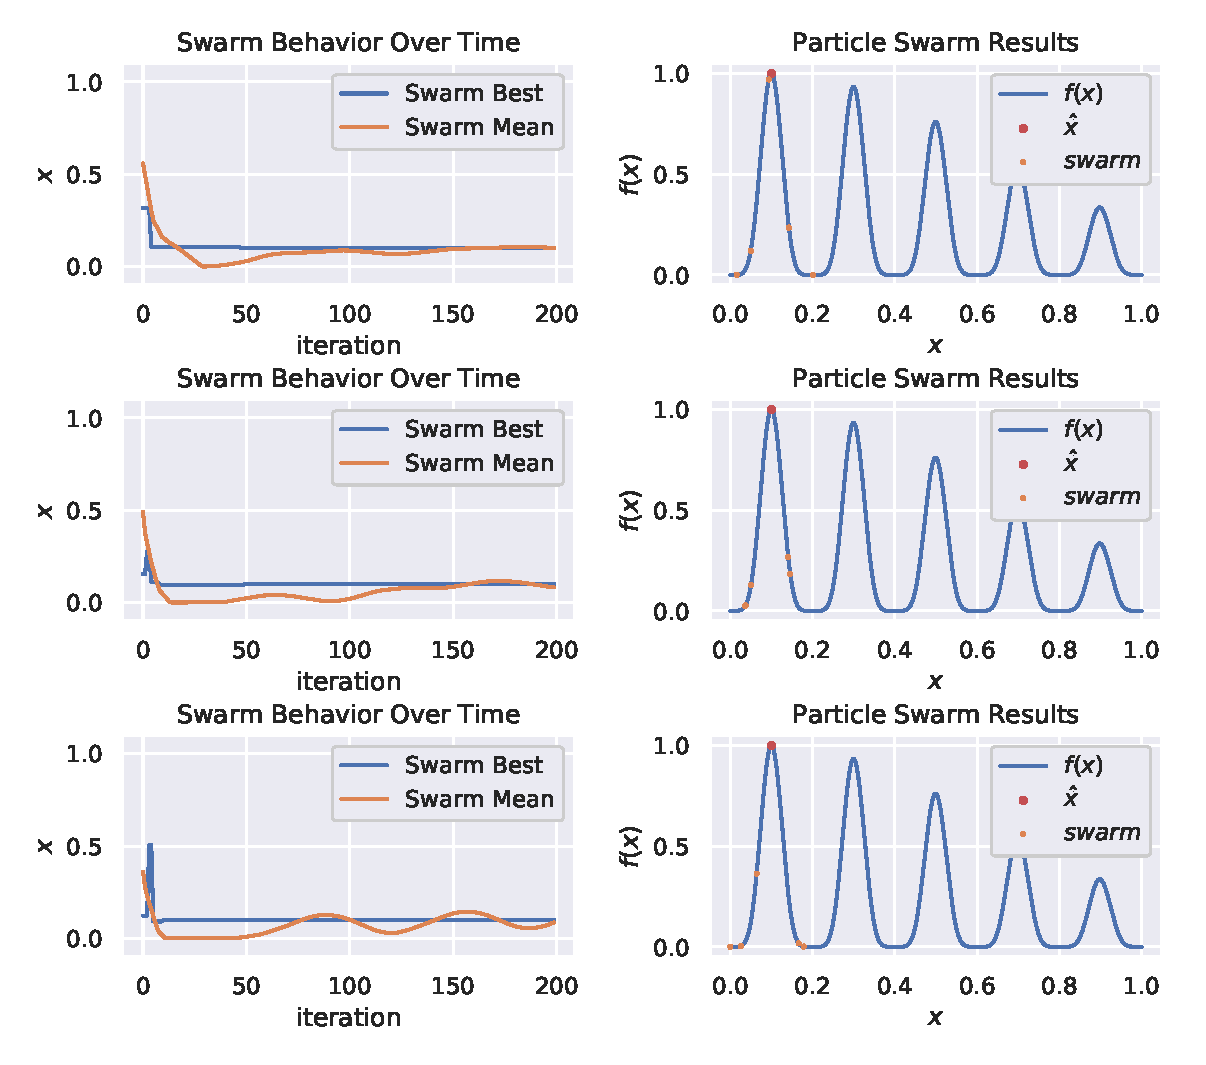
\includegraphics[width=\textwidth]{figures/pso/pso-tuned-vel-low-accel.eps}
    \caption{Tuned velocity, low acceleration.}\label{fig:pso:tuned-vel-low-accel}
\end{figure}

If we use the biased velocity limits to push the swarm to one side, we can see that it struggles to correct itself if the acceleration is lowered.

\begin{figure}[H]
    \centering
    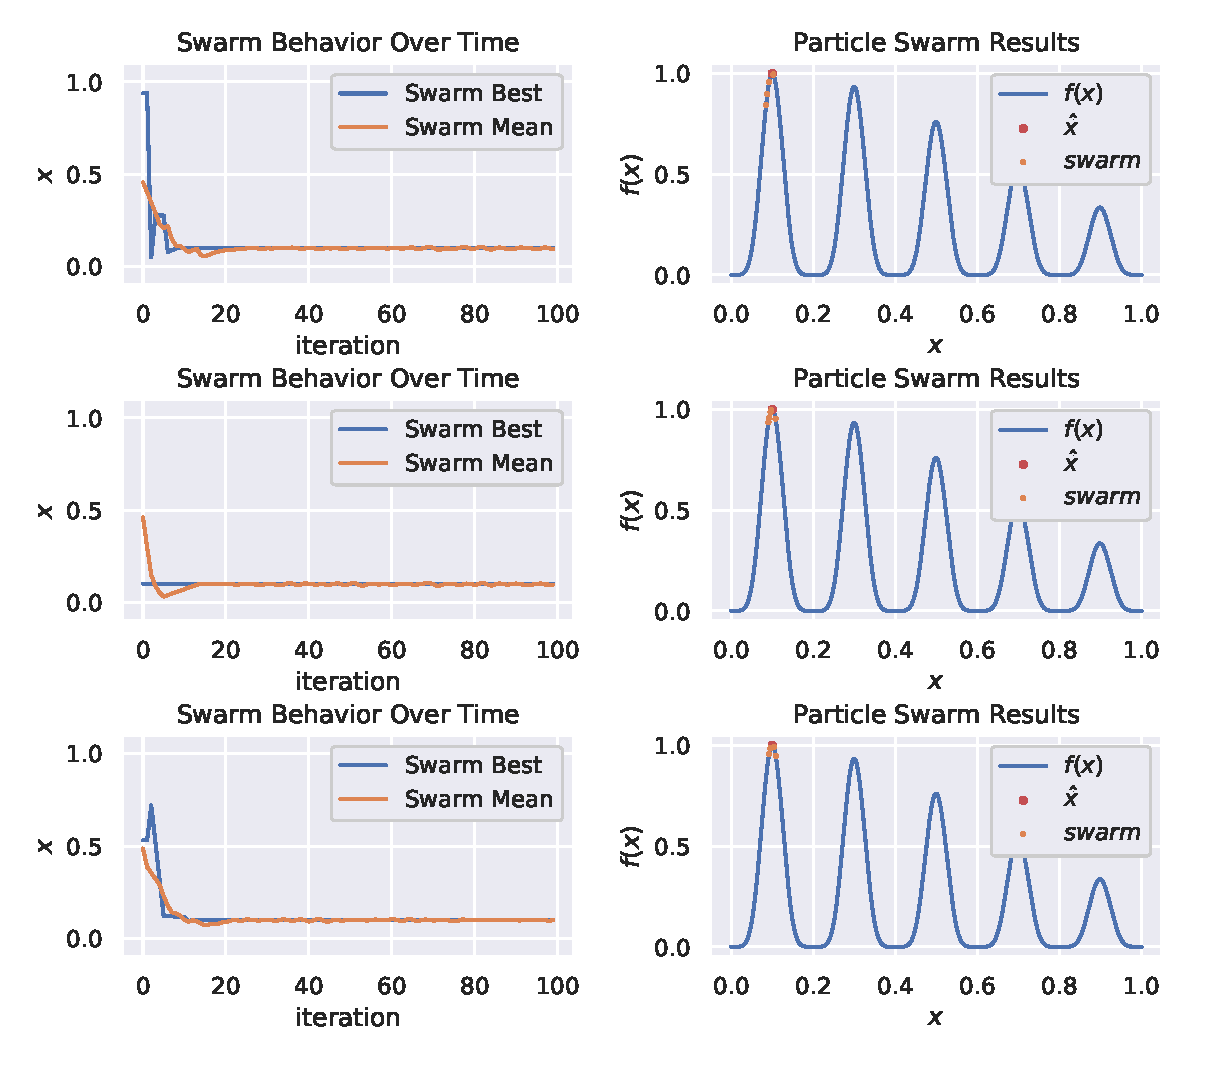
\includegraphics[width=\textwidth]{figures/pso/pso-tuned-vel-high-accel.eps}
    \caption{Tuned velocity, high acceleration.}\label{fig:pso:tuned-vel-high-accel}
\end{figure}

Our ultimate recommendation is to use global knowledge about the behavior of the function to push the swarm to one side or the other, yet to allow a high enough acceleration to correct any overshoots quickly.

This results in a stable swarm that does not move around much once it converges.

However, as \autoref{fig:pso:tuned-vel-bigger-domain} indicates, this only works if the optimum is to one side or the other of the feasible region.
In other cases, we must use equal left and right velocity biases.

\begin{figure}[H]
    \centering
    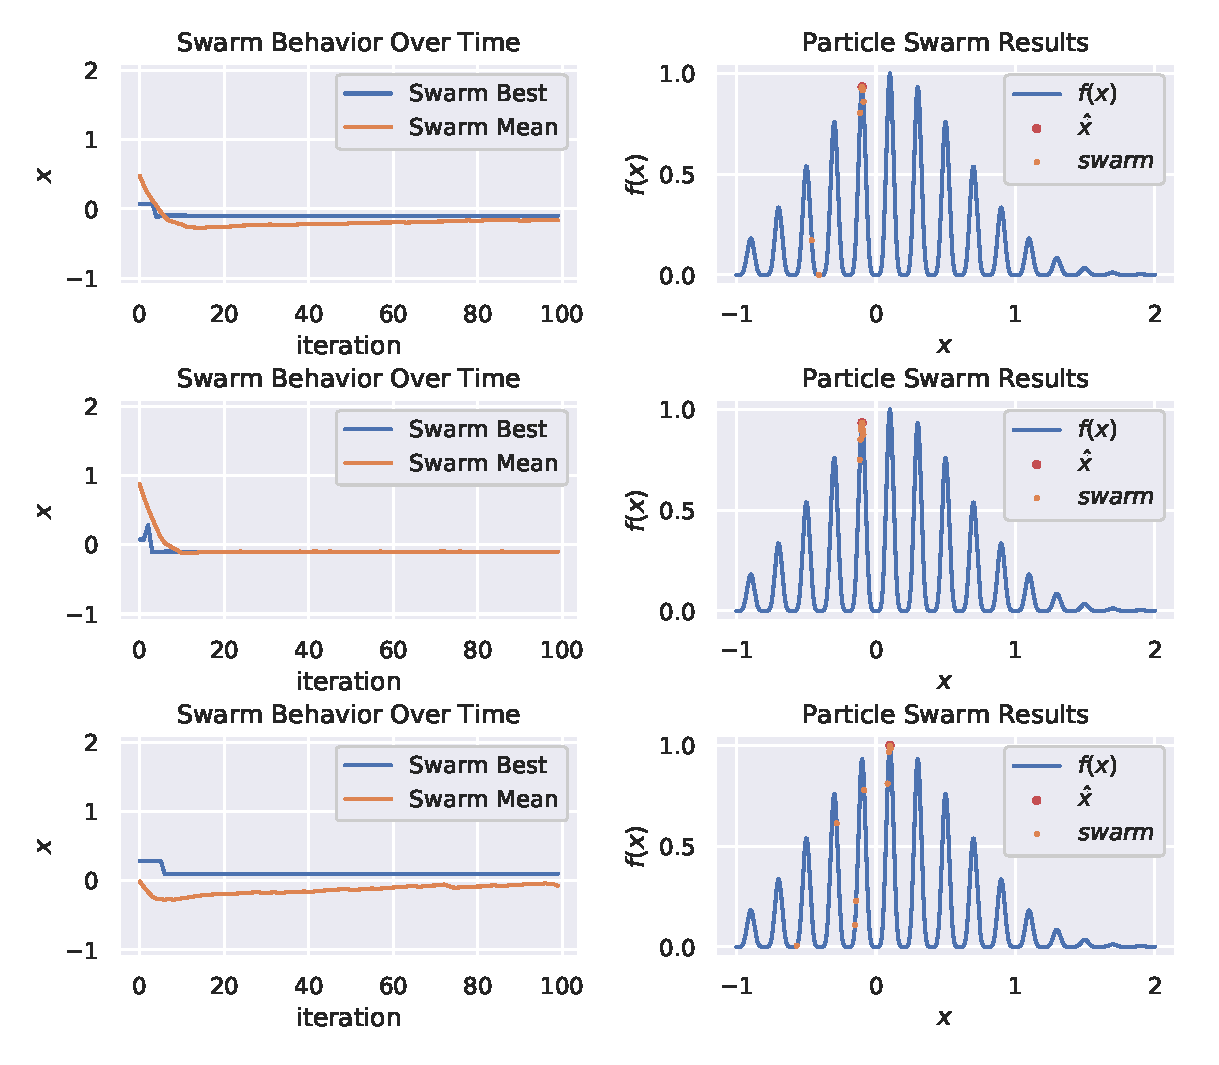
\includegraphics[width=\textwidth]{figures/pso/pso-tuned-vel-bigger-domain.eps}
    \caption{Tuned velocity, bigger domain}\label{fig:pso:tuned-vel-bigger-domain}
\end{figure}

\subsection{Conclusion}
We found that simulated annealing readily beat both other methods without much tuning.
It took a considerable amount of thought and effort to tune the particle swarm optimization algorithm before it would consistently converge to the same solution over multiple runs.
However, once tuned, it performed just as well as simulated annealing.
\end{document}
